
\documentclass[9pt]{beamer}
%\makeatletter
%\def\beamer@calltheme#1#2#3{%
%	\def\beamer@themelist{#2}
%	\@for\beamer@themename:=\beamer@themelist\do
%	{\usepackage[{#1}]{\beamer@themelocation/#3\beamer@themename}}}
%
%\def\usefolder#1{
%	\def\beamer@themelocation{#1}
%}
%\def\beamer@themelocation{}

%\usefolder{../config}

\usetheme[
block=fill,
titleformat=regular,
progressbar=frametitle
]{metropolis}
%\metroset[everytitleformat=regular] % regular, lowercase, uppercase ]
%\metroset[inner/block=fill]

%\setbeameroption{show notes} 
\usepackage{booktabs}
\usepackage[scale=2]{ccicons}

\usepackage{pgfplots}
\usepgfplotslibrary{dateplot}


%\ Hrvatski znakovi
\usepackage[utf8]{inputenc}
\usepackage[T1]{fontenc}
\usepackage[croatian]{babel}
\usepackage{todonotes}
\usepackage{amsmath}
\usepackage{amsfonts}
\selectlanguage{croatian} % american ngerman
\usepackage{todonotes}

% Koristenje Latin modern fonta
% Bez toga na nekim racunalima baca
% err: Font <taj i taj> at <mala velicina, npr4.0pt> not loadable: Metric (TFM) file not found. \end{frame}
\usepackage{lmodern}


\definecolor{RoyalBlue}{cmyk}{1, 0.50, 0, 0}
%\usepackage{natbib}
%\usepackage{bibentry}
\usepackage{scrextend}
\usepackage{hyperref}
%\usepackage[pdfa=true]{hyperref}
\hypersetup{%
    %draft, % = no hyperlinking at all (useful in b/w printouts)
    %colorlinks=true, 
    linktocpage=true, pdfstartpage=3, pdfstartview=FitV,%
    % uncomment the following line if you want to have black links (e.g., for printing)
    %colorlinks=false, linktocpage=false, pdfborder={0 0 0}, pdfstartpage=3, pdfstartview=FitV,% 
    breaklinks=true, pdfpagemode=UseNone, pageanchor=true, pdfpagemode=UseOutlines,%
    plainpages=false, bookmarksnumbered, bookmarksopen=true, bookmarksopenlevel=1,%
    hypertexnames=true, pdfhighlight=/O,%nesting=true,%frenchlinks,%
    %urlcolor=webbrown, linkcolor=RoyalBlue, citecolor=webgreen, %pagecolor=RoyalBlue,%
    %urlcolor=Blue, linkcolor=Blue, citecolor=Red, %pagecolor=Black,%
    %pdftitle={\myTitle},%
    %pdfauthor={\textcopyright\ \myName, \myUni, \myFaculty},%
    pdfsubject={},%
    pdfkeywords={},%
    pdfcreator={pdfLaTeX},%
    pdfproducer={LaTeX with hyperref and classicthesis}, %
    unicode = true 
} 

%\usepackage[pdftex]{graphicx}
% declare the path(s) where your graphic files are
\graphicspath{{./}{./figures/}}


\newcommand{\executeiffilenewer}[3]{%
	\ifnum\pdfstrcmp{\pdffilemoddate{#1}}%
	{\pdffilemoddate{#2}}>0%
	{\immediate\write18{#3}}\fi%
}
\newcommand{\includesvg}[1]{%
	\executeiffilenewer{#1.svg}{#1.pdf}%
	{inkscape -z -C --file=#1.svg %
		--export-pdf=#1.pdf --export-latex}%
	\input{#1.pdf_tex}%
}


% http://tex.stackexchange.com/questions/83882/how-to-highlight-python-syntax-in-latex-listings-lstinputlistings-command

\usepackage{listings}
\usepackage{color}
\usepackage[semibold]{sourcecodepro}

% Default fixed font does not support bold face
\DeclareFixedFont{\ttb}{T1}{txtt}{bx}{n}{12} % for bold
\DeclareFixedFont{\ttm}{T1}{txtt}{m}{n}{12}  % for normal
% Custom colors
\definecolor{deepblue}{rgb}{0,0,0.5}
\definecolor{deepred}{rgb}{0.6,0,0}
\definecolor{deepgreen}{rgb}{0,0.5,0}


% Python style for highlighting
\newcommand\pythonstyle{\lstset{
		language=Python,
		basicstyle=\small\ttfamily,
		otherkeywords={self},             % Add keywords here
		keywordstyle=\small\ttfamily\color{deepblue},
		emph={MyClass,__init__},          % Custom highlighting
		emphstyle=\small\ttfamily\color{deepred},    % Custom highlighting style
		stringstyle=\color{deepgreen},
		frame=tb,                         % Any extra options here
		showstringspaces=false            % 
	}}
	
	
	% Python environment
	\lstnewenvironment{python}[1][]
	{
		\pythonstyle
		\lstset{#1}
	}
	{}
	
	% Python for external files
	\newcommand\pythonexternal[2][]{{
			\pythonstyle
			\lstinputlisting[#1]{#2}}}
	
	% Python for inline
	\newcommand\pythoninline[1]{{\pythonstyle\lstinline!#1!}}

% \includeonlyframes{current}

%\documentclass[ucs]{beamer}
%\usetheme[menuwidth={0.3\paperwidth}]{erlangen}
%\setbeamercovered{transparent=20} 

\usepackage{amsmath,amsfonts,amsthm,amssymb}
\usepackage{setspace}
\usepackage{Tabbing}
\usepackage{fancyhdr}
\usepackage{lastpage}
\usepackage{extramarks}
\usepackage{chngpage}
\usepackage{soul,color}
\usepackage{graphicx,float,wrapfig}
\usepackage{xcolor}
\usepackage[normalem]{ulem}
\usepackage{mathtools}

\definecolor{erlangenlyellow}{RGB}{123, 25, 121}
%\usepackage[utf8x]{inputenc}
%\usepackage{default}
%\usepackage[T1]{fontenc}

\usepackage{verbatim}
\usepackage{listings}


\usepackage{subcaption}
\usepackage{lmodern}

\title{Teksture i protočni sustav}

% \subtitle{ Yet, it doesn't seem so clear to me anymore…?}
\subtitle {And so it was told, and so I told myself}
\institute{Računalna grafika}


\begin{document}
\begin{frame}
 \titlepage
\end{frame}

%\begin{frame}{Sadržaj}
%  \tableofcontents
%  % You might wish to add the option [pausesections]
%\end{frame}
% \section{Uvod}
\section{Protočni sustav}
\begin{frame}{Protočni sustav}
	\begin{center}
		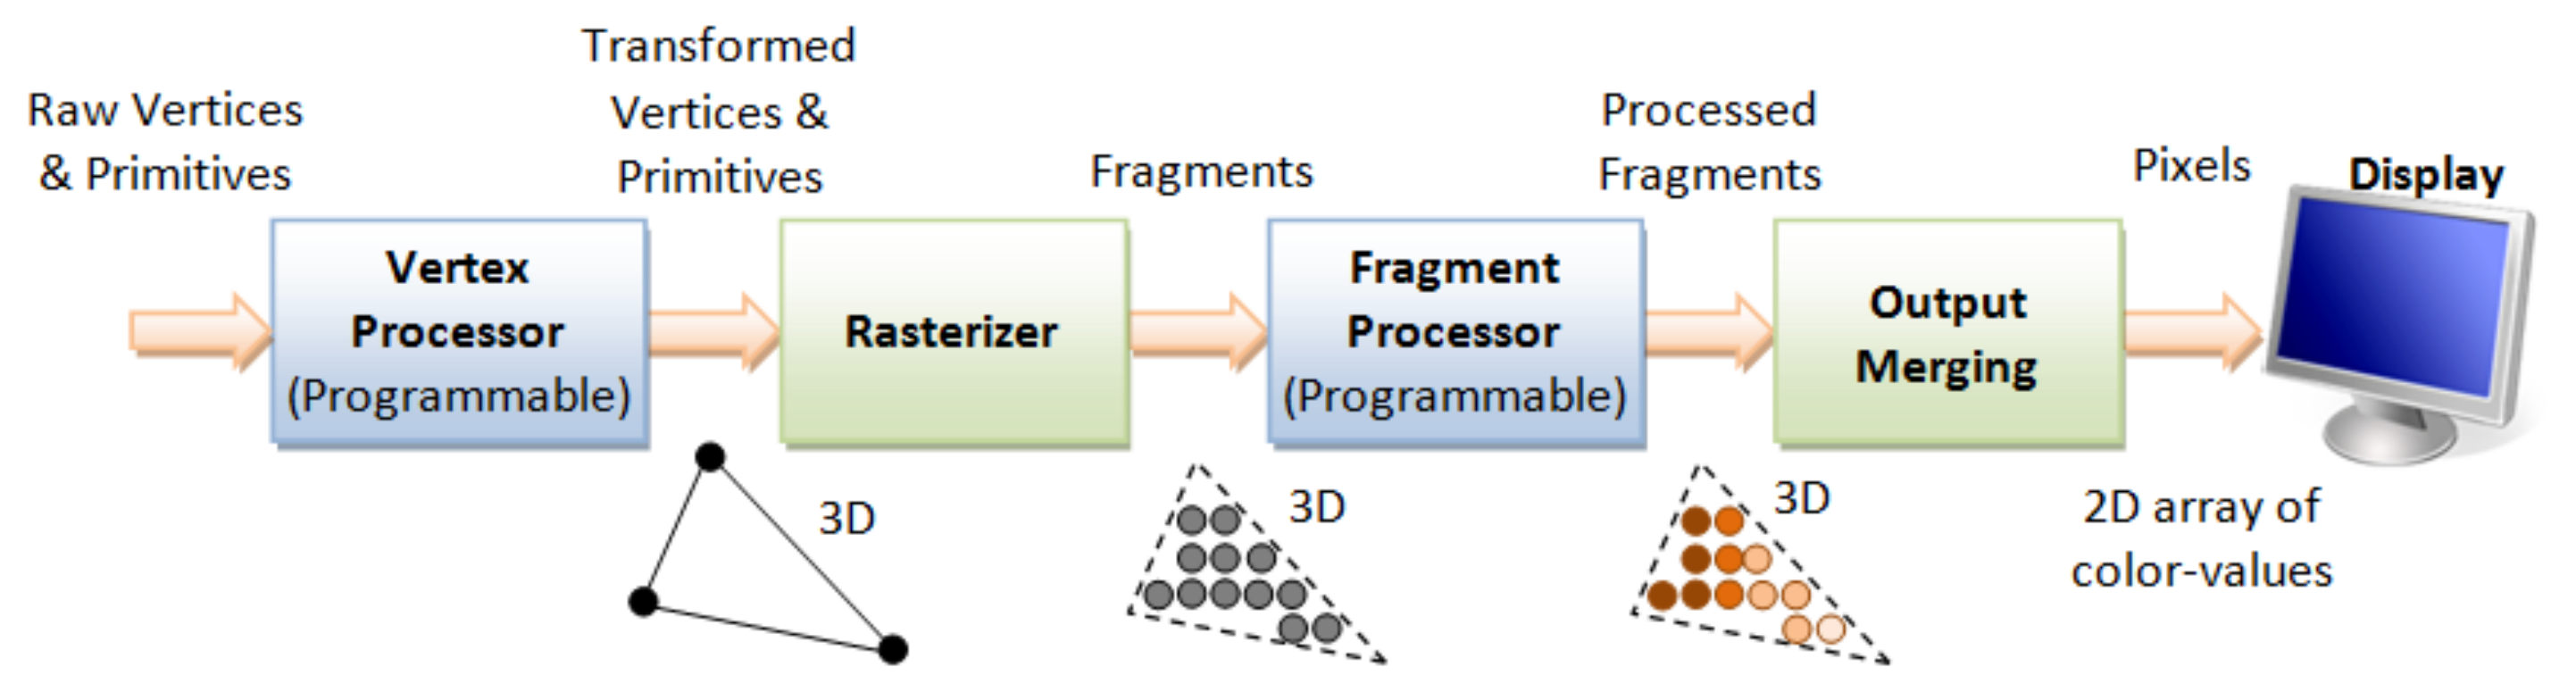
\includegraphics[width=10cm]{./slike/graphics_pipeline_01.png}
	\end{center}
\begin{itemize}
	\item Vertex Processing: Procesiranje i transformacija verteksa i normala
	\item Rasterizacija: Konverzija svakog primitiva (povezanih verteksa) u set fragmenata. Fragment, ugrubo: pikel s atributima (položaj, boja, normala i tekstura)
	\item Fragment Processing: Procesiranje fragmenata
	\item Output Merging: Spajanje fragmenata svih primitiva iz 3D u 2D color-pixel za prikaz
\end{itemize}
\end{frame}


\begin{frame}{Protočni sustav}
	\begin{center}
		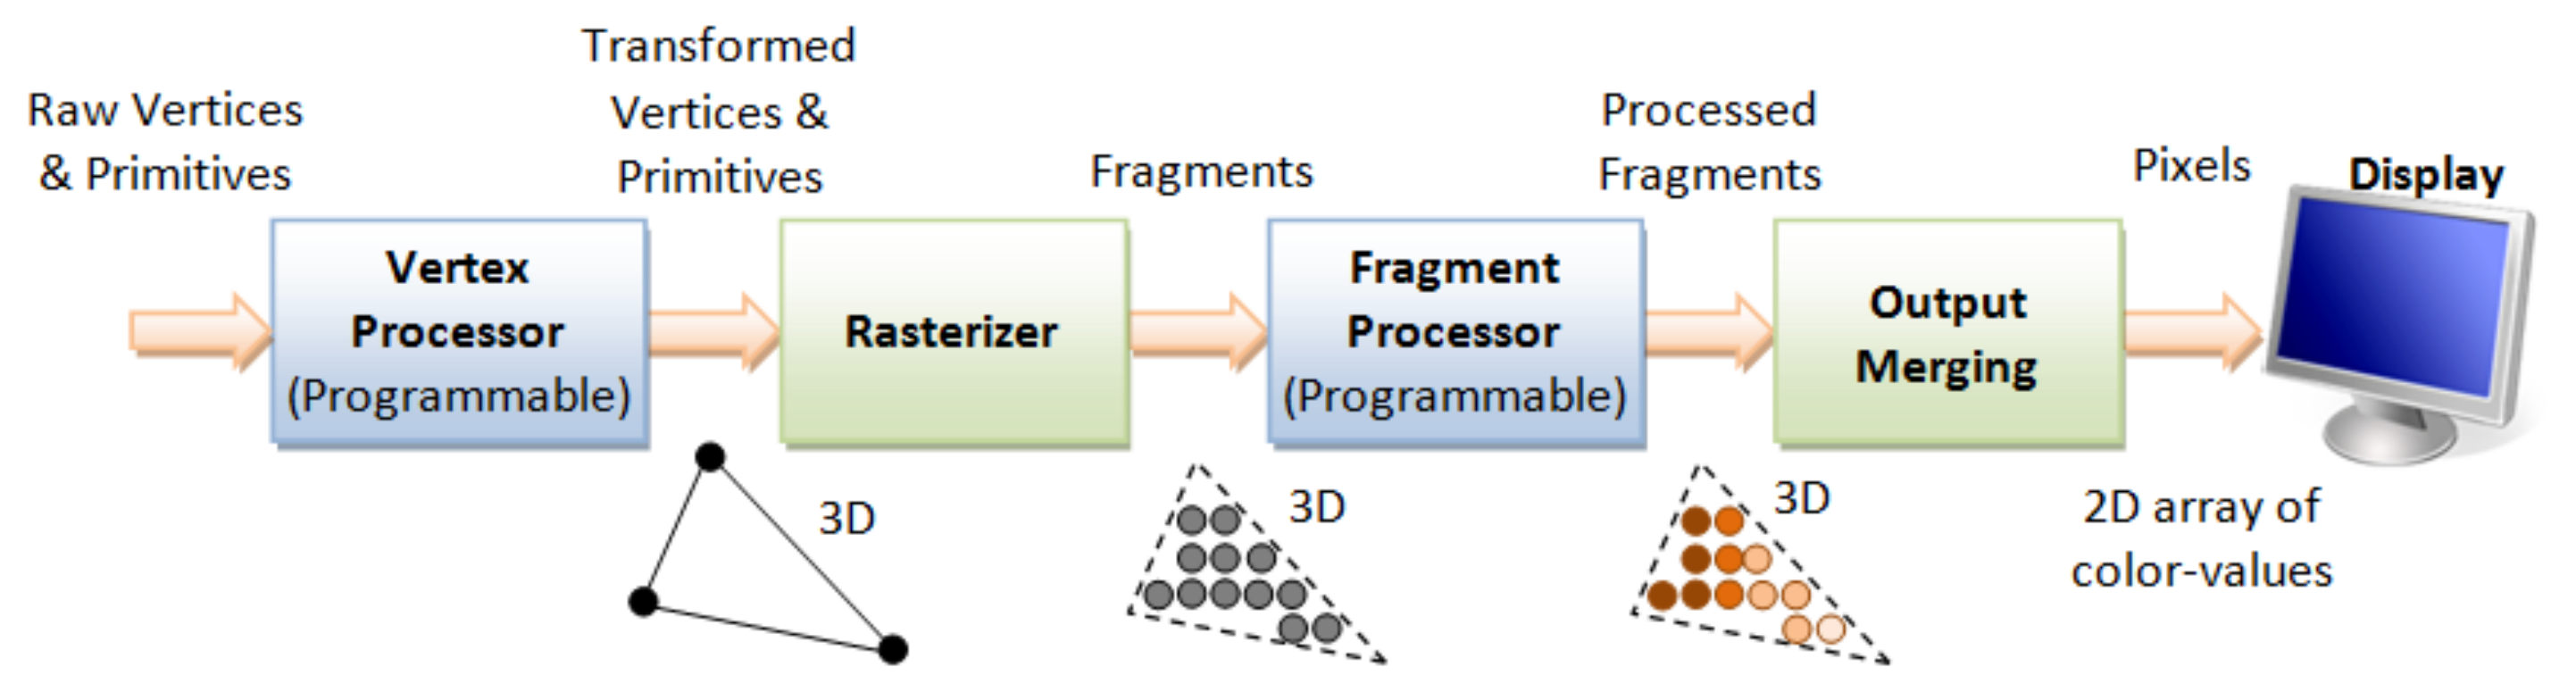
\includegraphics[width=10cm]{./slike/graphics_pipeline_01.png}
	\end{center}
	\begin{itemize}
		\item Vertex Processing: vertex shader: transformacije i osvjetljavanje za svaki verteks
		\item Fragment processor: fragment shader: teksture i osvjetljavanje za svaki fragment
	\end{itemize}
\end{frame}

\begin{frame}{Pixel vs fragment}
	\begin{center}
		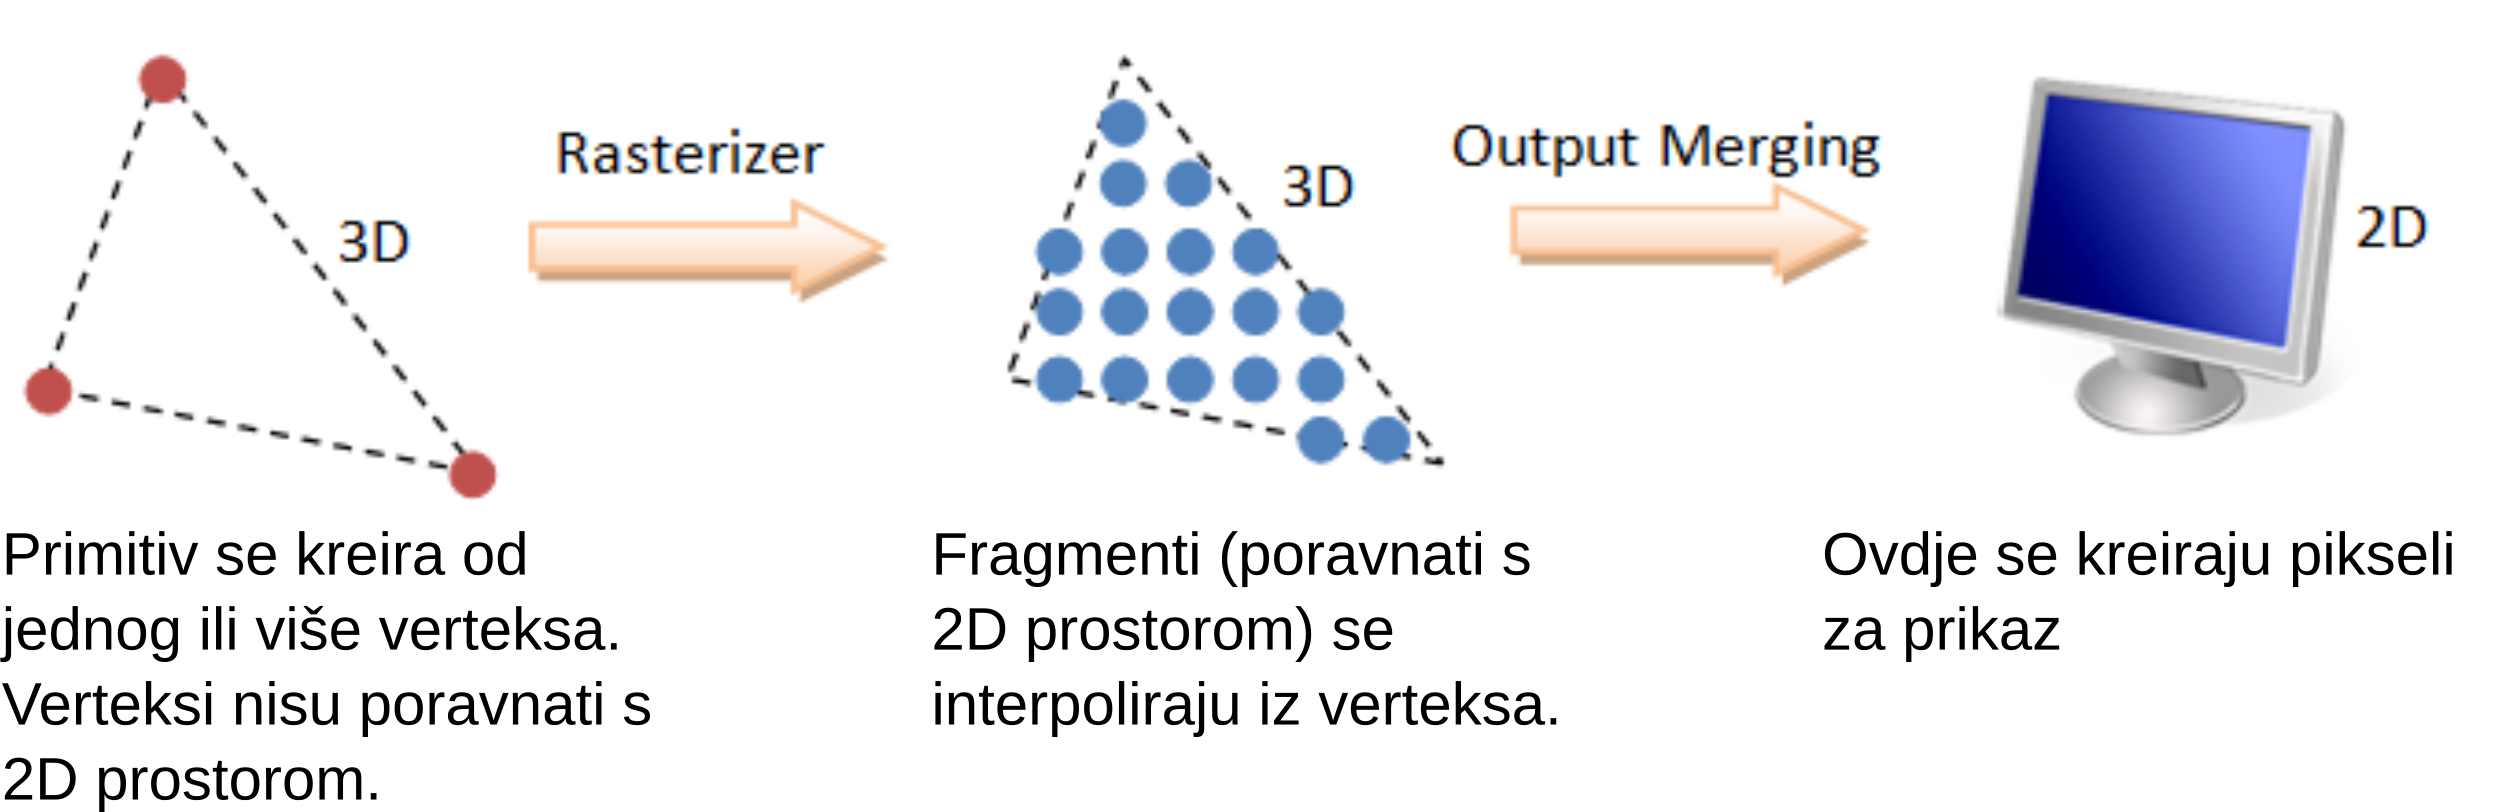
\includegraphics[width=6cm]{./slike/graphics_pipeline_02.png}
	\end{center}
\end{frame}

\begin{frame}{Protočni sustav}
	\begin{center}
		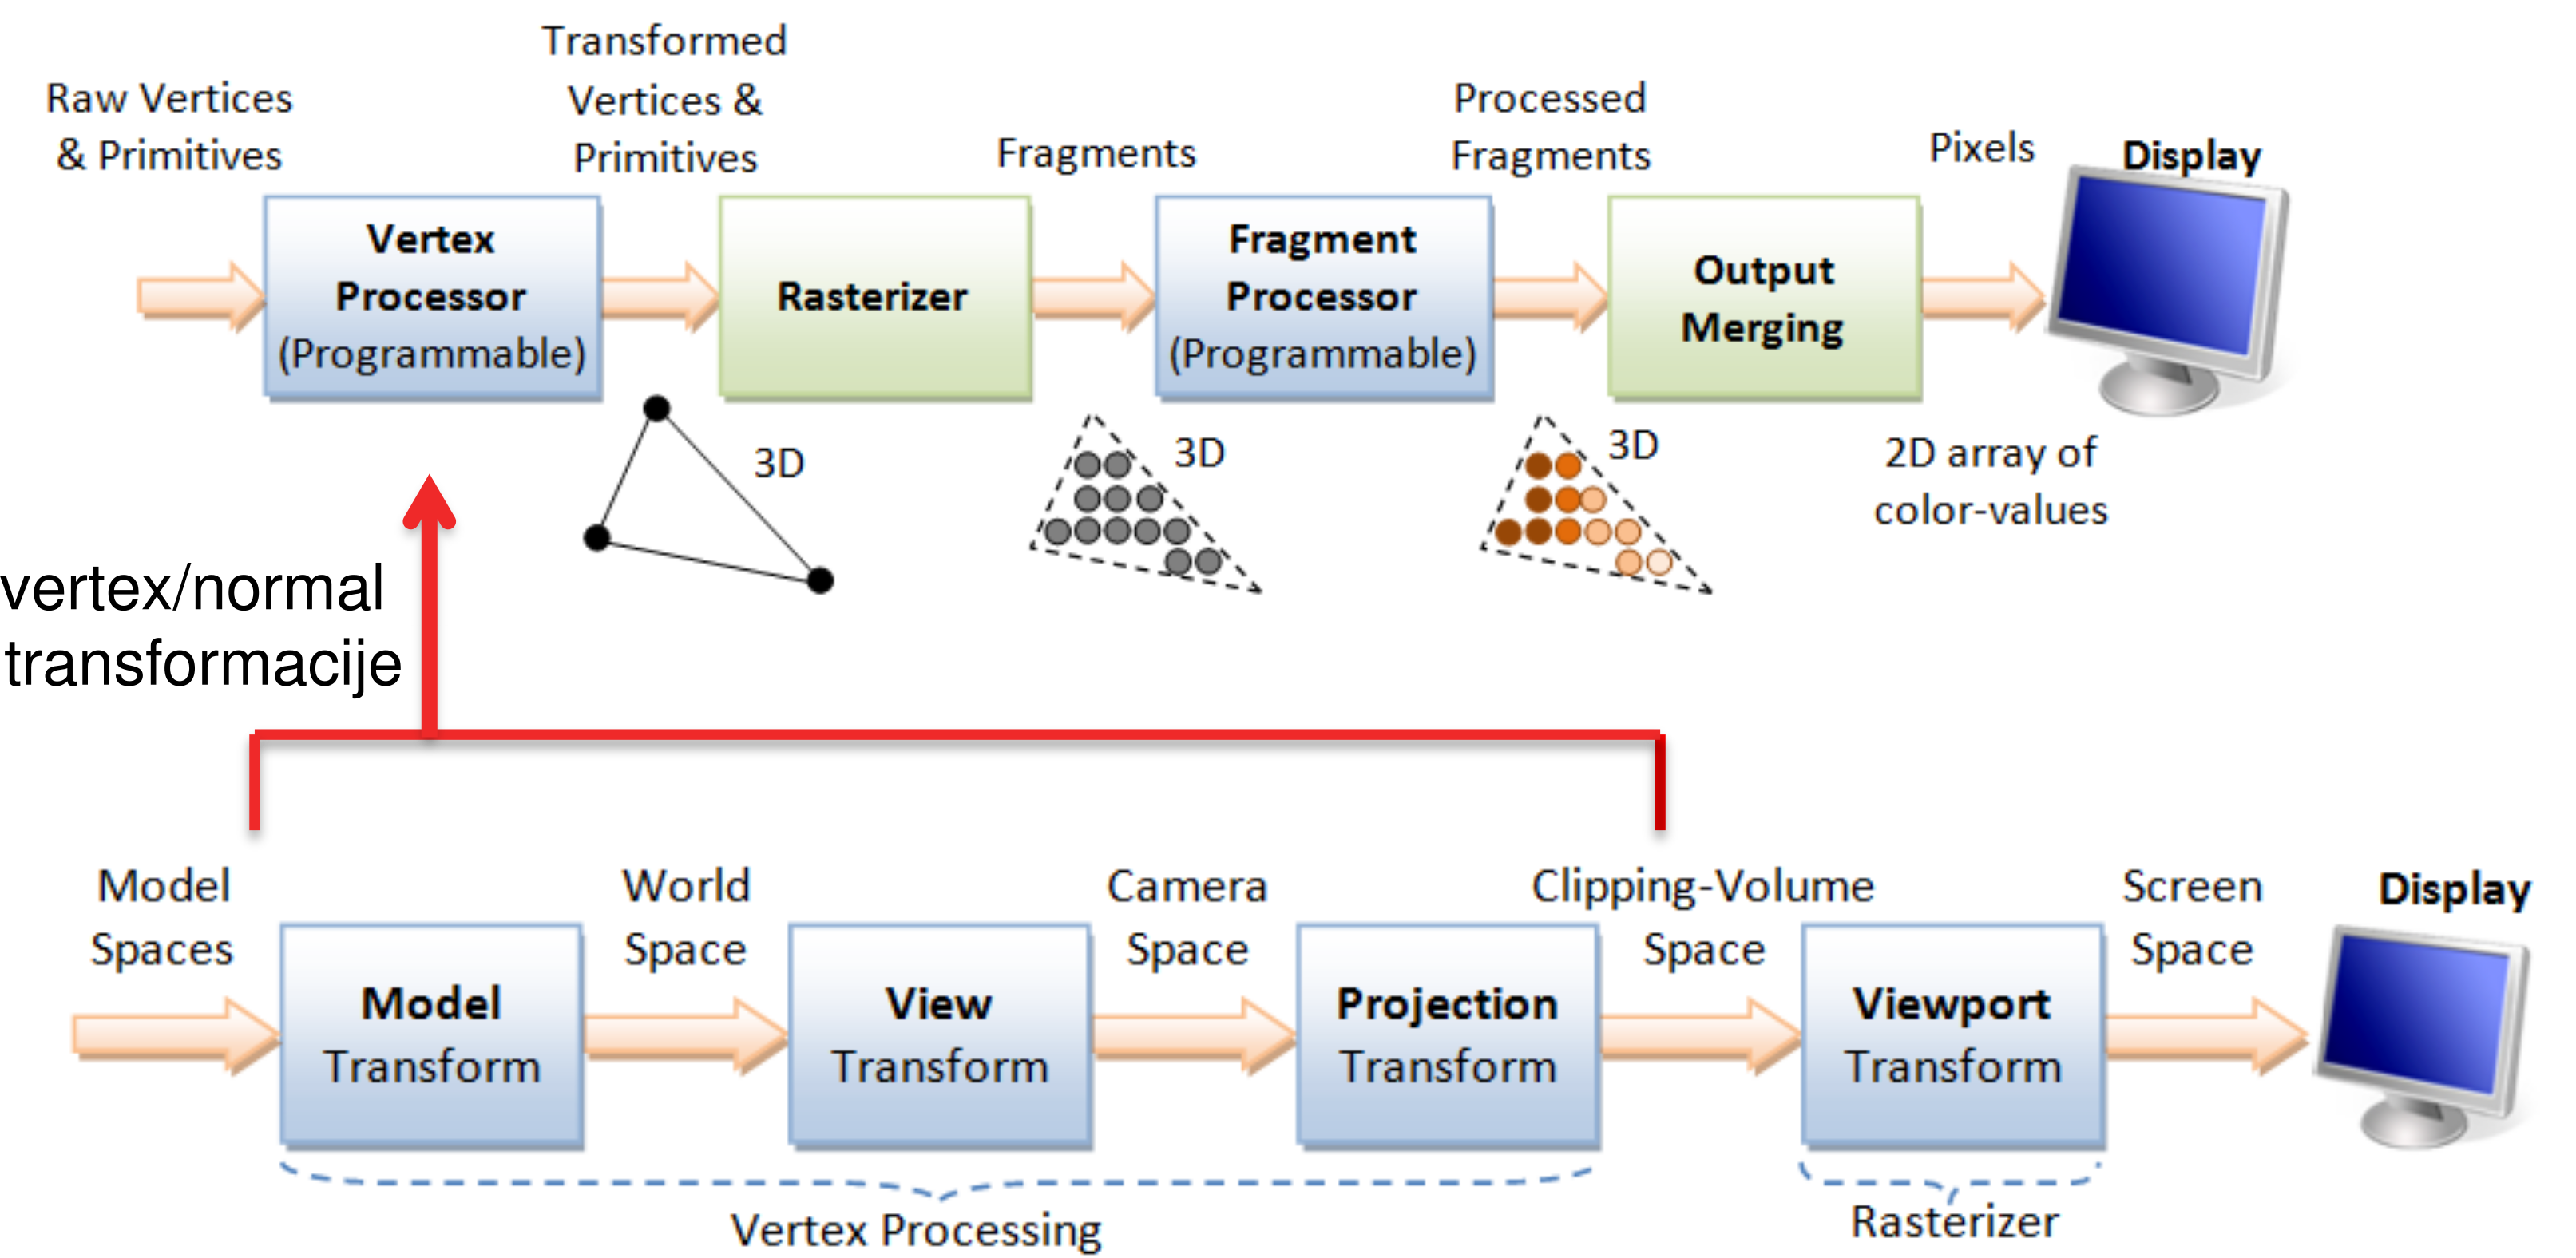
\includegraphics[width=10cm]{./slike/graphics_pipeline_03.png}
	\end{center}
\end{frame}

\begin{frame}{Protočni sustav}
	\begin{center}
		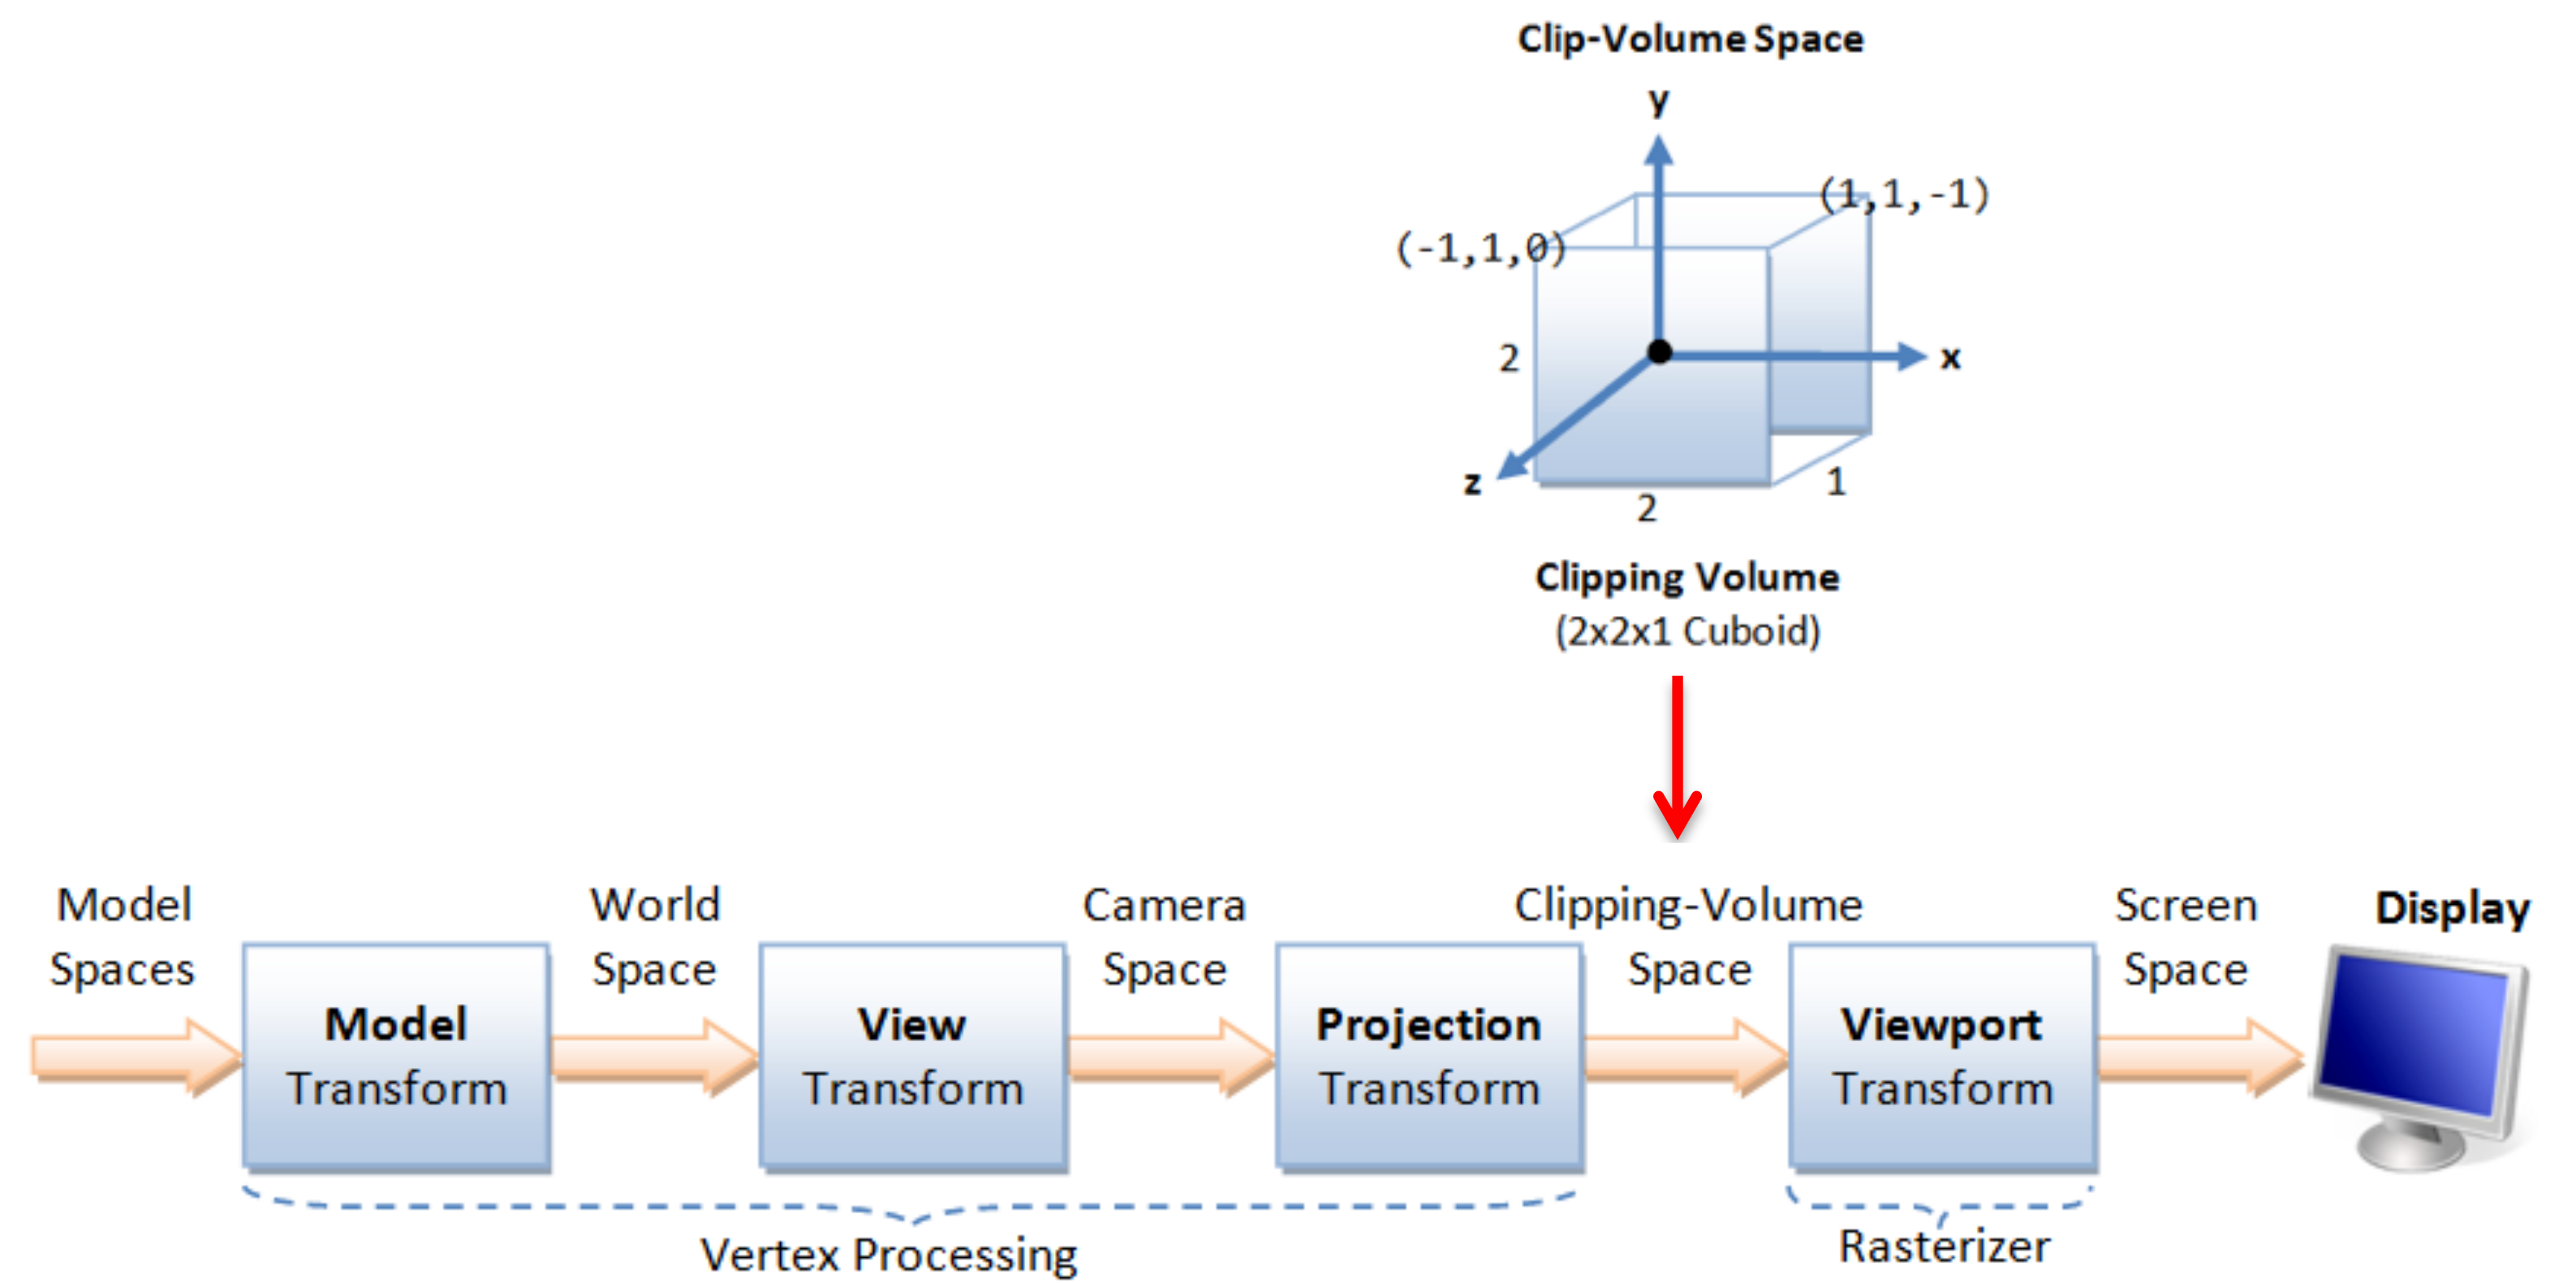
\includegraphics[width=10cm]{./slike/graphics_pipeline_04.png}
	\end{center}
\end{frame}

\begin{frame}{Protočni sustav i shaders}
	\begin{center}
		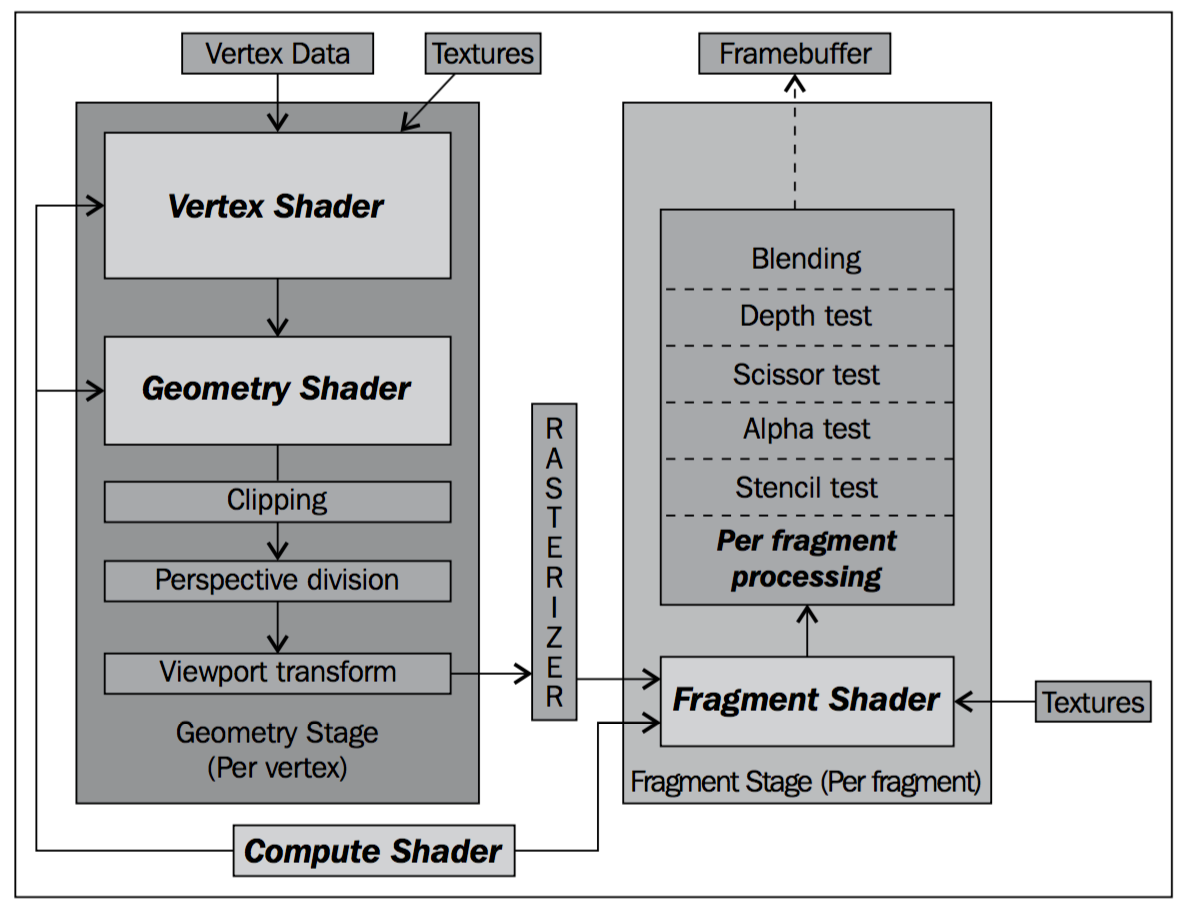
\includegraphics[width=8cm]{./slike/graphics_pipeline_05.png}
	\end{center}
\end{frame}

\section{Teksture}
\begin{frame}{Protočni sustav i teksture}
	\begin{center}
		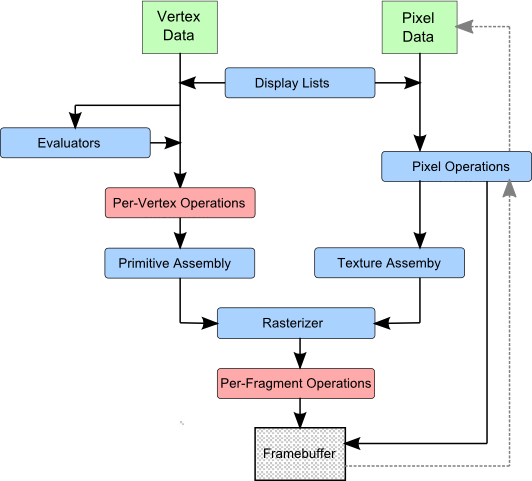
\includegraphics[width=8cm]{./slike/graphics_pipeline_06.png}
	\end{center}
\end{frame}

\begin{frame}{Primjer sa dva trokuta}
	\begin{center}
		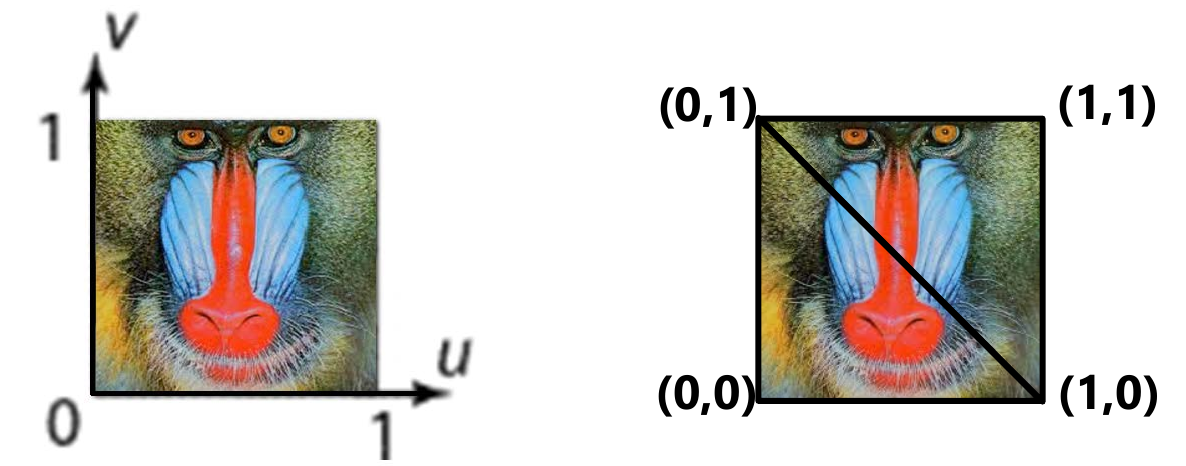
\includegraphics[width=8cm]{slike/baboon.png}
	\end{center}
	\begin{itemize}
		\item Postaviti teksturu na dva trokuta
		\item  Svaki verteks trokuta ima pridodanu $(u,v)$ koordinatu, čime je onda poznato koji dio teksture se treba pridodati na koji trokut
		\item Preslikava se (R,G,B) boja teksture za svaki piksel unutar trokuta
	\end{itemize}
\end{frame}

\begin{frame}{Teksture}
	\begin{center}
		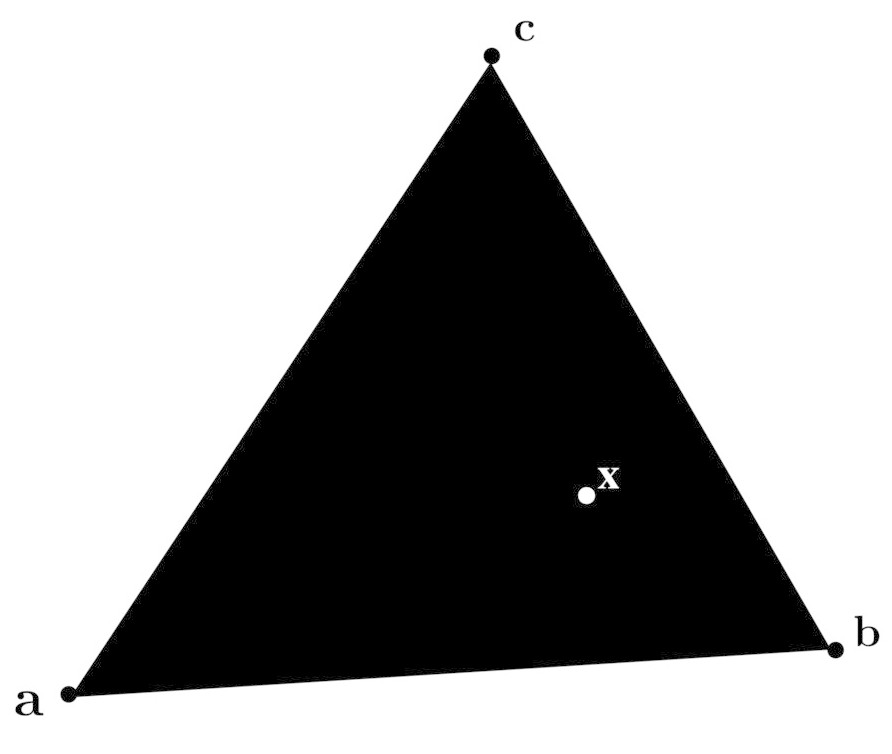
\includegraphics[width=6cm]{./slike/slide_023.jpg}
	\end{center}
\end{frame}

\begin{frame}{Teksture}
	\begin{center}
		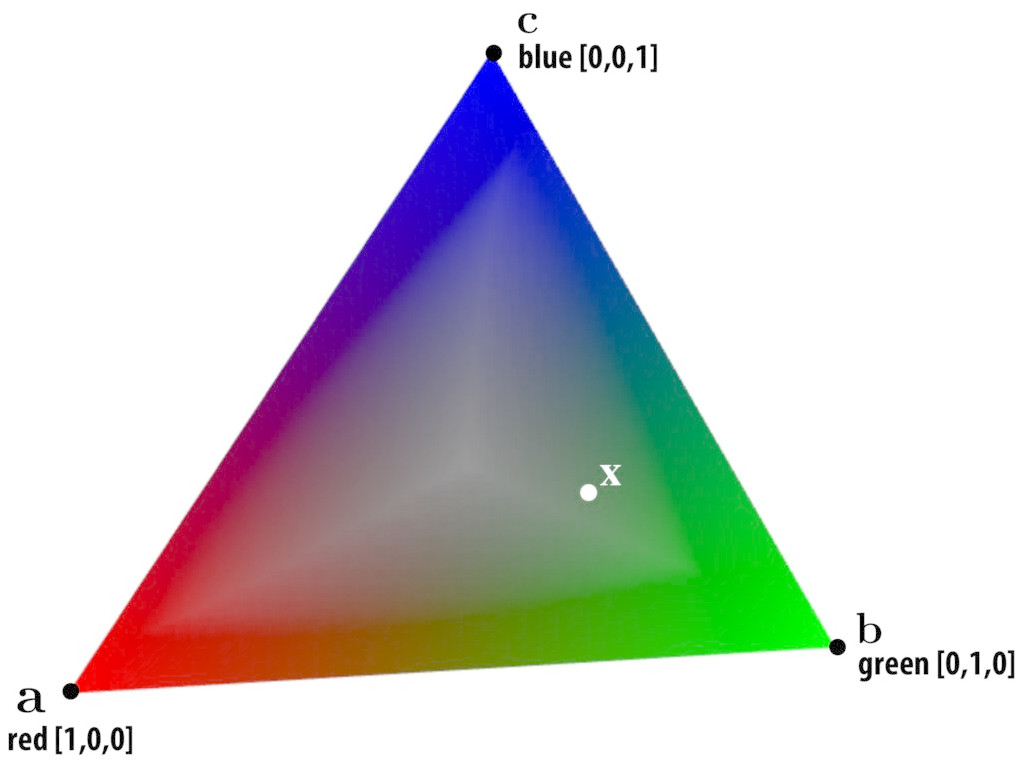
\includegraphics[width=6cm]{./slike/slide_024.jpg}
	\end{center}
\end{frame}


\begin{frame}{Teksture}
	\begin{center}
		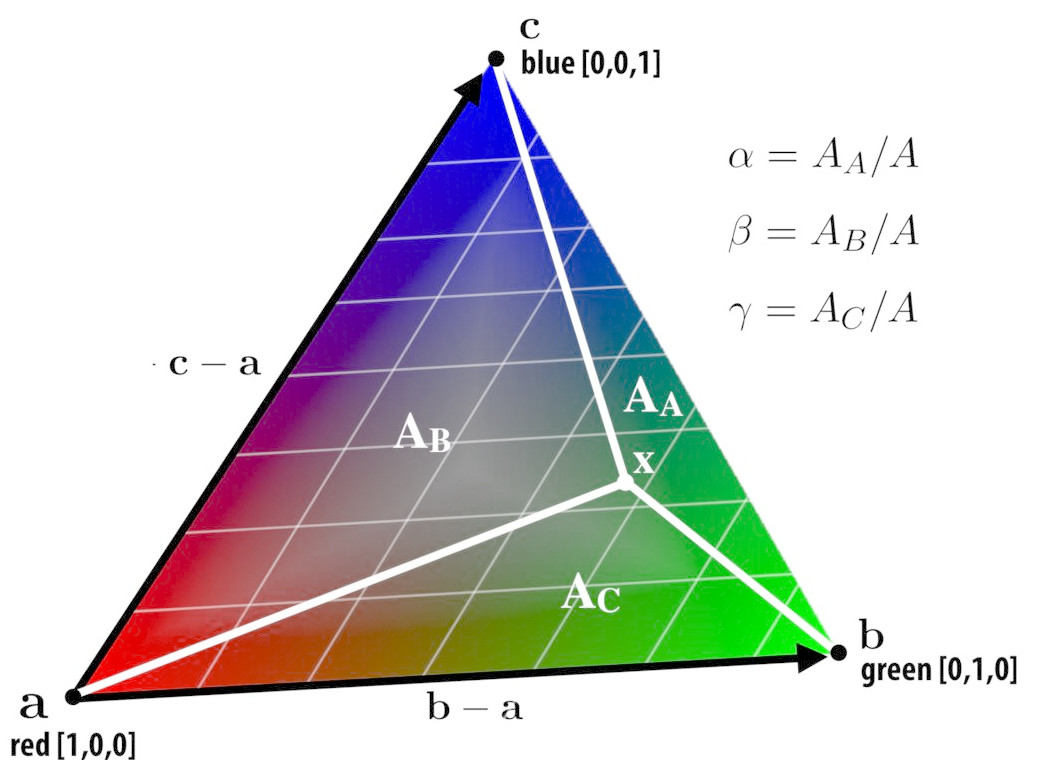
\includegraphics[width=6cm]{./slike/slide_029.jpg}
	\end{center}
\end{frame}

\begin{frame}{Teksture}
	\begin{block}{Algoritam}
		\texttt{for each covered screen sample (x,y):}\\
		\texttt{\ (u,v) = eval texcoord val at (x,y):}\\
		\texttt{\ float3 texcolor = texture.sample(u,v);} \\
	\end{block}
\end{frame}

\begin{frame}{Texture coordinate function}
	\begin{block}{Texture coordinate function}
		\begin{itemize}
			\item Ključno: naći odgovarajuću poziciju u koordinatnom sustavu teksture (slike) koja odgovara poziciji unutar poligona
			\item Potrebno definirati funkciju preslikavanja "od poligona do teksture" koja se lako može izračunati za svaki piksel.
		\end{itemize}
	\end{block}
	\begin{center}
		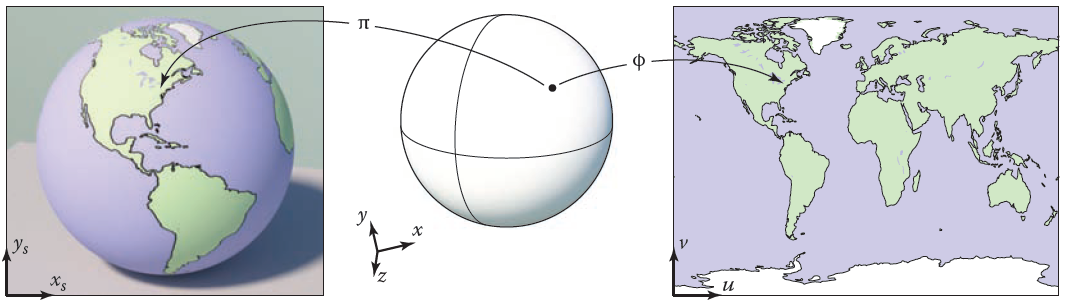
\includegraphics[width=9cm]{slike/texture_coo_fun.png}
	\end{center}
	Na isti način na koji \textit{projekcija} pogleda $\pi$ preslikava svaku točku na površinu objekta $\mathbf{S}$ na točku na slici, \textit{Texture coordinate function} $\psi$ preslikava svaku točku na površini objekta na točku na teksturi $\mathbf{T}$. Time je definicija takve funkcije $\phi$ fundamentalna za sve primjene preslikavanja teksture.
\end{frame}

\begin{frame}{Texture coordinate function}
	\begin{block}{Zadaća funkcije}
		\begin{itemize}
			\item Dodijeliti koordinate teksture svakoj točki/poziciji na površini.
		\end{itemize}
		\begin{align*}
		\phi &: S \rightarrow T \\
		& : (x, y, z) \mapsto (u, v)
		\end{align*}
	\end{block}
	\begin{block}{T}
		\begin{itemize}
			\item \textit{texture space}
			\item obično pravokutnik sa slikom
			\item jedinični pravokutnik $(u, v) \in  \left[0, 1\right]^2$
		\end{itemize}
	\end{block}
	tldr: $\phi$ preslikava vrijednosti sa površine na teksturu.
\end{frame}

\begin{frame}{Kako izgleda funkcija?}
	\begin{block}{Primjer}
		Ako je površina pravokutna, $z=const.$, poravnata sa $x$ i $y$ osima: 
		\begin{align*}
		u = ax \quad v = by
		\end{align*}
	\end{block}
	\begin{enumerate}
		\item Dodijeliti koordinate teksture $(s, t)$ točki $(x,y,z)$
		\item Koristiti vrijednost piksela teksture (textela) koji je najbliži $(u, v)$ kao vrijednost teksture na $x, y$
	\end{enumerate}
	
	\begin{center}
		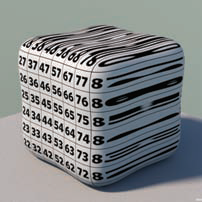
\includegraphics[width=3cm]{slike/planar_proj.png}
	\end{center}
	Gornja funkcija je loš izbor: što ako se površina rotira? Ako je velika? Perspektiva?
\end{frame}

\begin{frame}{Kakva treba biti funkcija?}
	\begin{block}{Svojstva funkcije $\phi$}
		\begin{itemize}
			\item Bijektivnost
			\item Deformacija veličine - $|\phi'|$ ne bi trebao značajno varirati - bliske točke na objektu bi se trebale preslikati na bliske točke na teksturi
			\item Deformacija oblika - $\phi'$ se ne bi trebao jako mijenjati u različitim smjerovima - krug se ne bi trebao preslikavati u jako izduženu elipsu
		\end{itemize}
	\end{block}
\end{frame}

\begin{frame}{Protočni sustav, teksture}
	\begin{itemize}
		\item Određivanje pozicije na poligonu (object space)
		\begin{itemize}
			\item Koordinate teksture su definirane za pozicije na poligonu
			\item Tekstura se giba zajedno sa  objektom 
		\end{itemize}
		\item Projekcijska funkcija, O i S preslikavanje
		\begin{itemize}
			\item Preslikava 3D poziciju na poligonu na 2D vrijednost 
		\end{itemize}
		\item Corresponder funkcija
		\begin{itemize}
			\item preslikavanje iz parametarskog prostora u prostor teksture
			\item  transformacija $(u, v)$ u raspon od 0 so 1: repeat, clamp, mirror, clamp to edge, clamp to border
			\item Sada se mogu dobiti vrijednosti iz teksture
		\end{itemize}
		\item Transformacija vrijednosti, blending funkcije
		\begin{itemize}
			\item Funkcija koja transformira dobivene vrijednosti teksture, matrice transformacije u homogenom obliku
			\item definiranje načina uporabe teksture:
			\begin{itemize}
				\item zamjena boje s bojom teksture
				\item linearna kombinacija boje objekta s bojom teksture
				\item množenje, dodavanje, oduzimanje boje objekta i teksture
				\item izračun modela osvjetljavanja
			\end{itemize}
		\end{itemize}
	\end{itemize}
\end{frame}

\begin{frame}{Preslikavanje teksture}
	\begin{block}{Preslikavanje slike na površinu objekta}
		\begin{itemize}
			\item Tekstura se definira u ortogonalnom $(u, v)$ koordinatnom sustavu
			\item Površina (na koju se lijepi tekstura) se definira u nekom drugom koordinatnom sustavu $(x,y,z)$ na način da se svaka koordinata zadaje preko parametarske funkcije:  $x(s,t)$, $y(s,t)$, $z(s,t)$.
			\item Potrebno odrediti funkciju preslikavanja između parametarskog prostora i prostora teksture: $s = f(u,v)$, $t = g(u,v)$
			\item Inverzno preslikavanje: $u = F(s,t)$, $v = G(s,t)$
		\end{itemize}		
	\end{block}	
\end{frame}

\begin{frame}{S preslikavanje}
	\begin{block}{Sfera}
		\begin{itemize}
			\item $(u,v)=(2p/C,2q/C)\rightarrow (\theta, \phi)$
			\item gdje su $\theta, \phi$ sferne koordinate
			\item $C = 1+\sqrt{1+p^2+q^2}$,
			\item $p=\tan(\theta)\cos(\phi)$ , $q=\tan(\theta)\cos(\phi)$
			
		\end{itemize}
	\end{block}
	\begin{center}
		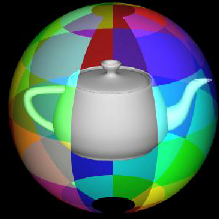
\includegraphics[height=3.4cm]{slike/teksture_kugla_01.png}
		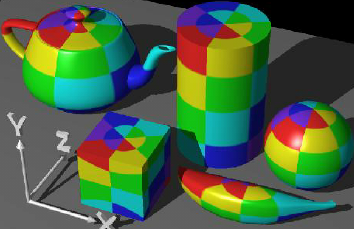
\includegraphics[height=3.4cm]{slike/teksture_kugla_02.png}
	\end{center}
\end{frame}
%
\begin{frame}{S preslikavanje - ravnina}
	$$ f(p) = (p_{x}/a, p_{y}/b)$$ 
	\begin{center}
		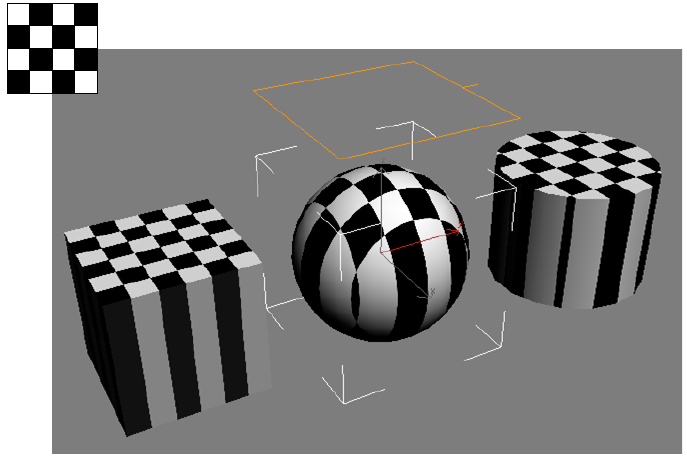
\includegraphics[width=8cm]{slike/02_projekcije_planar.png}
	\end{center}
\end{frame}

\begin{frame}{S preslikavanje - cilindar}
	$$ f(p) = (\phi, p_{y}/h)$$ 
	\begin{center}
		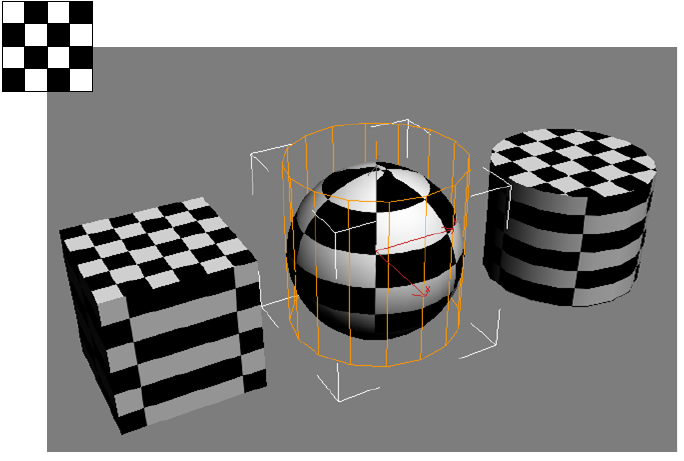
\includegraphics[width=8cm]{slike/02_projekcije_cylindrical.png}
	\end{center}
\end{frame}
%
\begin{frame}{S preslikavanje - sfera}
	$$ f(p) = (\phi, \theta)$$ 
	\begin{center}
		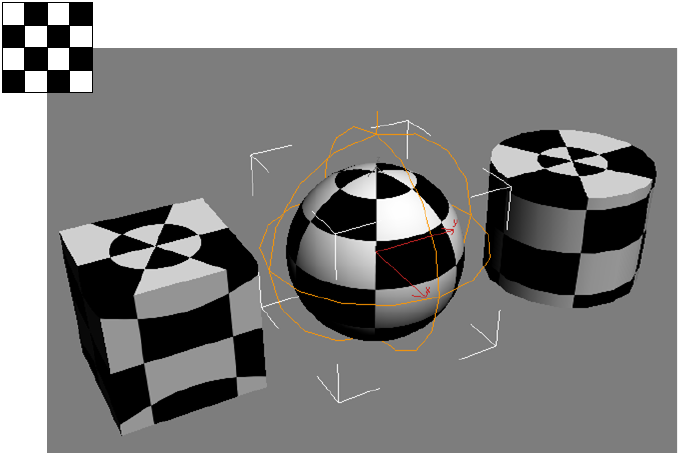
\includegraphics[width=8cm]{slike/02_projekcije_spherical.png}
	\end{center}
\end{frame}

\begin{frame}{S preslikavanje - kocka}
	
	\begin{center}
		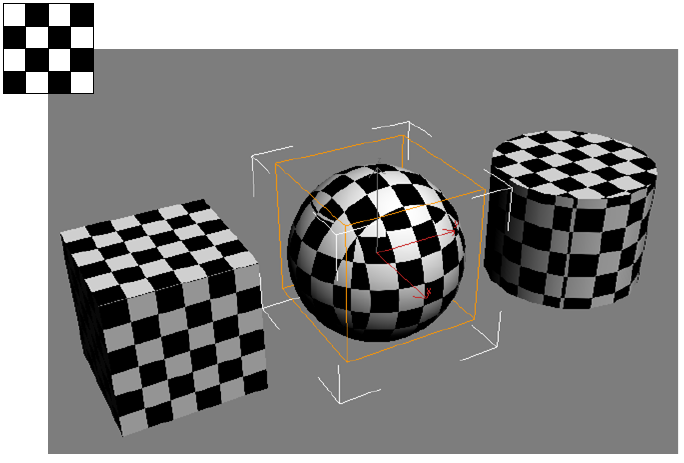
\includegraphics[width=5cm]{slike/02_projekcije_cubical.png}
	\end{center}
	\begin{center}
		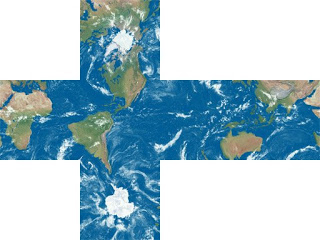
\includegraphics[width=5cm]{slike/earthcube_cross.jpg}
	\end{center}
\end{frame}
%
\begin{frame}{ O preslikavanje}
	\begin{block}{Četiri tehnike preslikavanja na objekt}
		\begin{itemize}[<+->]
			\item Reflektirana zraka - Reflection
			\only<1-2>{\begin{itemize}
					\item Prati zraku od očišta do objekta i prati rezultirajuću reflektiranu zraku od
					objekta do površine - \textit{environmental mapping}
					\begin{center}
						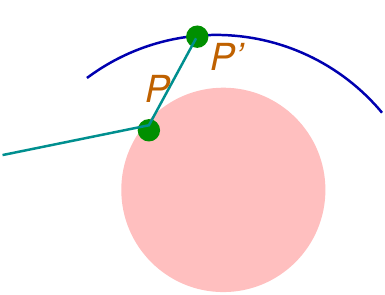
\includegraphics[width=3cm]{slike/reflektirana_zraka.png}
					\end{center}
			\end{itemize}}
			\item Normala objekta - position
			\only<3>{\begin{itemize}
					\item Naći presjek normale objekta i plohe
					\begin{center}
						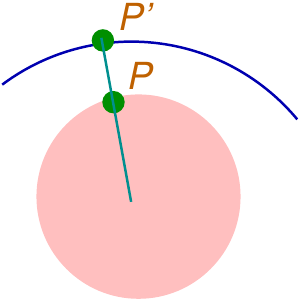
\includegraphics[width=3cm]{slike/normala_objekta.png}
					\end{center}
			\end{itemize}}
			\item Centroid objekta - centroid
			\only<4>{\begin{itemize}
					\item Presjecište linije definirane centroidom objekta i točke na površini objekta s prijelaznom plohom
					\begin{center}
						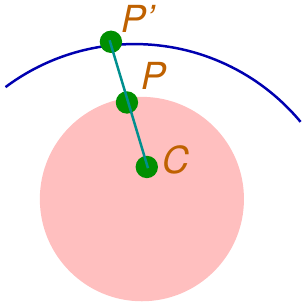
\includegraphics[width=3cm]{slike/centroid_objekta.png}
					\end{center}
			\end{itemize}}
			\item Normala prijelazne površine - surface normal
			\only<5>{\begin{itemize}
					\item Praćenje zrake u smjeru normale u točki prijelazne plohe da bi se našao presjek s objektom
					\begin{center}
						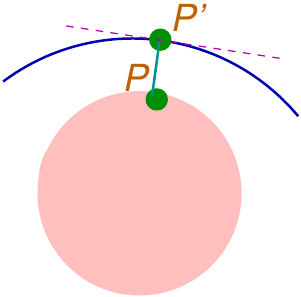
\includegraphics[width=3cm]{slike/normala_prijelazne_povrsine.png}
					\end{center}
			\end{itemize}}
			\item Normala objekta i centroid objekta su loša ideja ako je prijelazna površina cilindar. 
		\end{itemize}
	\end{block}
\end{frame}
%
\begin{frame}{Kombinacije preslikavanja}
	3 \textbf{O preslikavanja} x 4 \textbf{S preslikavanja} = 12 kombinacija
	
	\begin{center}
		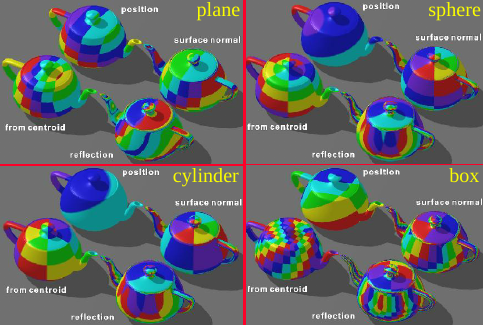
\includegraphics[width=10cm]{slike/02_SO_mapping_primjeri.png}
	\end{center}
\end{frame}
%

\section{Bump i displacement preslikavanje}
\begin{frame}{Bump mapping}
	\begin{block}{Problemi}
		\begin{itemize}
			\item Dodavanje teksture na glatku površinu rezultira glatkom površinom.
			\item Korištenje grube teksture u cilju prikaza grube površine nije dobra ideja.
			\item Grube površine bi trebale imati dodanu malu nasumičnu komponentu u normali, a time i u smjeru refleksije svjetla.
		\end{itemize}
	\end{block}
	\begin{itemize}
		\item Perturbacija normale površine
		\item Za svaku točku na površini $\mathbf{S}$, parcijalne derivacije su $\mathbf{S}_u$ i $\mathbf{S}_v$. 
		\item Odnosno: $\mathbf{n} = \mathbf{S}_u \times\mathbf{S}_v$
	\end{itemize}
\end{frame}	
%
\begin{frame}{Bump mapping}
	\begin{block}{}
		Nova ploha je definirana sa $S'(u,v) = S(u,v) + P(u,v)\frac{n}{|n|}$ \\
		gdje je $P(u,v)$ funkcija perturbacije u smjeru normale osnovne plohe, zadaje se analitički ili tablično\\
		Rezultirajuća normala je $\mathbf{n'} = \mathbf{S'}_{u} \times \mathbf{S'}_{v}$ 
	\end{block}
	
	\begin{block}{Konačno}
		$$n' = n + \frac{P_{u}(\mathbf{n} \times \mathbf{S}_{v})}{|n|} + \frac{P_{v}(\mathbf{S}_{u} \times \mathbf{n})}{|n|}$$
	\end{block}
\end{frame}
%
\begin{frame}{Bump mapping contd.}
	
	\begin{columns}[t]
		\begin{column}{7cm}
			\begin{center}
				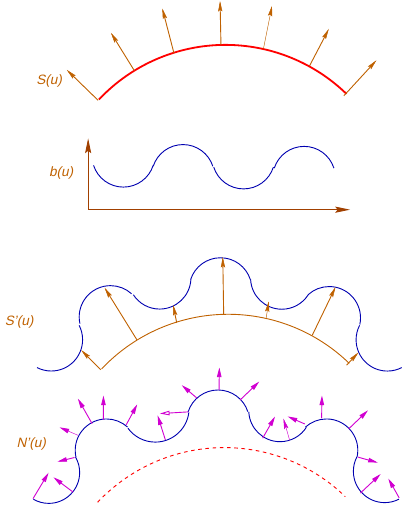
\includegraphics[width=5cm]{slike/03_bump_mapping.png}
			\end{center}
		\end{column}
		\begin{column}{5cm}
			\begin{center}
				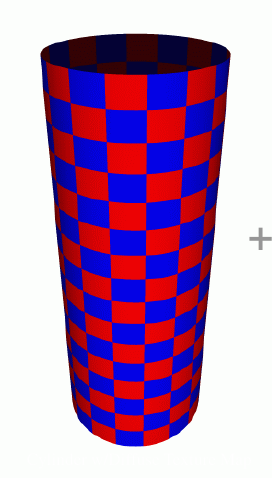
\includegraphics[width=1.8cm]{slike/bump_01.png}
				
\includegraphics[width=1.8cm]{slike/bump_02.png}
				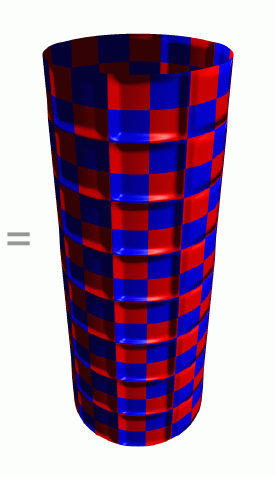
\includegraphics[width=1.8cm]{slike/bump_03.png}
			\end{center}
			\begin{center}
				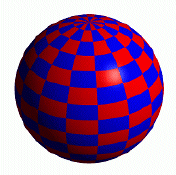
\includegraphics[width=1.8cm]{slike/bump_01_01.png}
				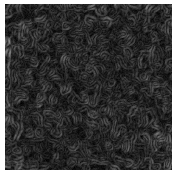
\includegraphics[width=1.8cm]{slike/bump_02_02.png}
				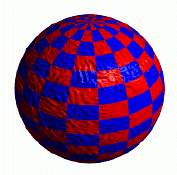
\includegraphics[width=1.8cm]{slike/bump_03_03.png}
			\end{center}
		\end{column}
	\end{columns}
\end{frame}
%
\begin{frame}{Displacement mapping}
	Vrijednosti teksture su vrijednosti pomaka geometrije u smjeru normale.
	\begin{center}
		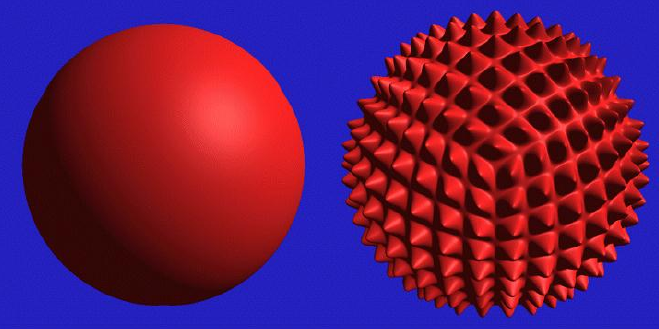
\includegraphics[width=2.5cm]{slike/displacement_map.png}
	\end{center}
	\begin{block}{}
		Bump mapping općenito ne zahtijeva puno resursa. Displacement mapping zahtijeva više resursa tijekom
		inicijalizacije i manipulacije, ali kako se računanje odvija tijekom postavljanja scene, ne povećava vrijeme renderiranja, dok bump mapping povećava vrijeme renderiranja iz razloga što pokreće novi shader proces.
	\end{block}
	
	
\end{frame}
%
\begin{frame}{Bump vs Displacement mapping}
	\begin{block}{Primjena Displacement mapping}
		\begin{itemize}
			\item tereni
			\item animacija travnatih i šumovitih područja
			\item valovi vodenih i sličnih površina
			\item animacija vatre, dima, oblaka ili sličnih čestičnih volumena
		\end{itemize}
	\end{block}
	
	\begin{block}{Primjena Bump mapping}
		\begin{itemize}
			\item realizam tekstura - koža itd.
			\item dodavanje malih detalja objektu
		\end{itemize}
	\end{block}
\end{frame}
%
\begin{frame}{Bump vs Displacement mapping contd.}
	\begin{center}
		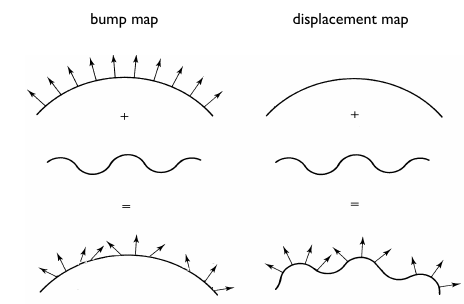
\includegraphics[width=10cm]{slike/03_bump_vs_displacement_mapping.png}
	\end{center}
\end{frame}

\begin{frame}{Bump vs Displacement mapping contd.}
	\begin{center}
		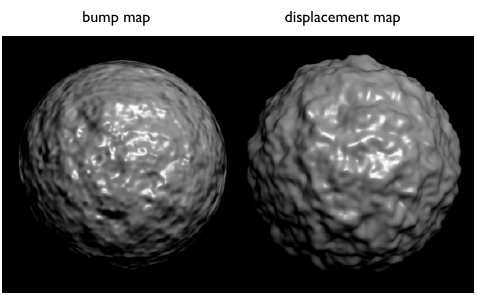
\includegraphics[width=10cm]{slike/03_bump_vs_displacement_mapping_a.png}
	\end{center}
\end{frame}
\section{Problemi}
\begin{frame}{Teksture}
	\begin{center}
		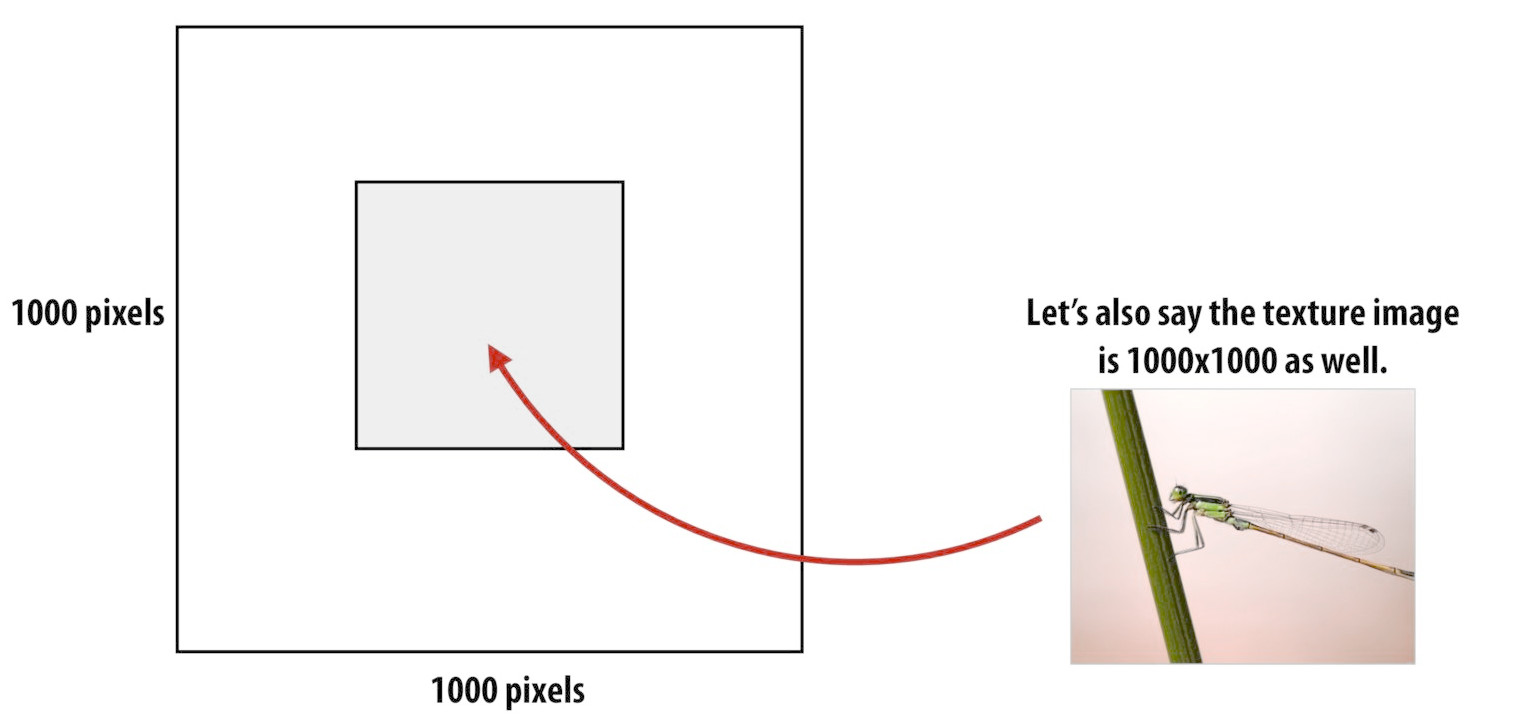
\includegraphics[width=8cm]{./slike/slide_050.jpg}
	\end{center}
\end{frame}

\begin{frame}{Teksture}
	\begin{center}
		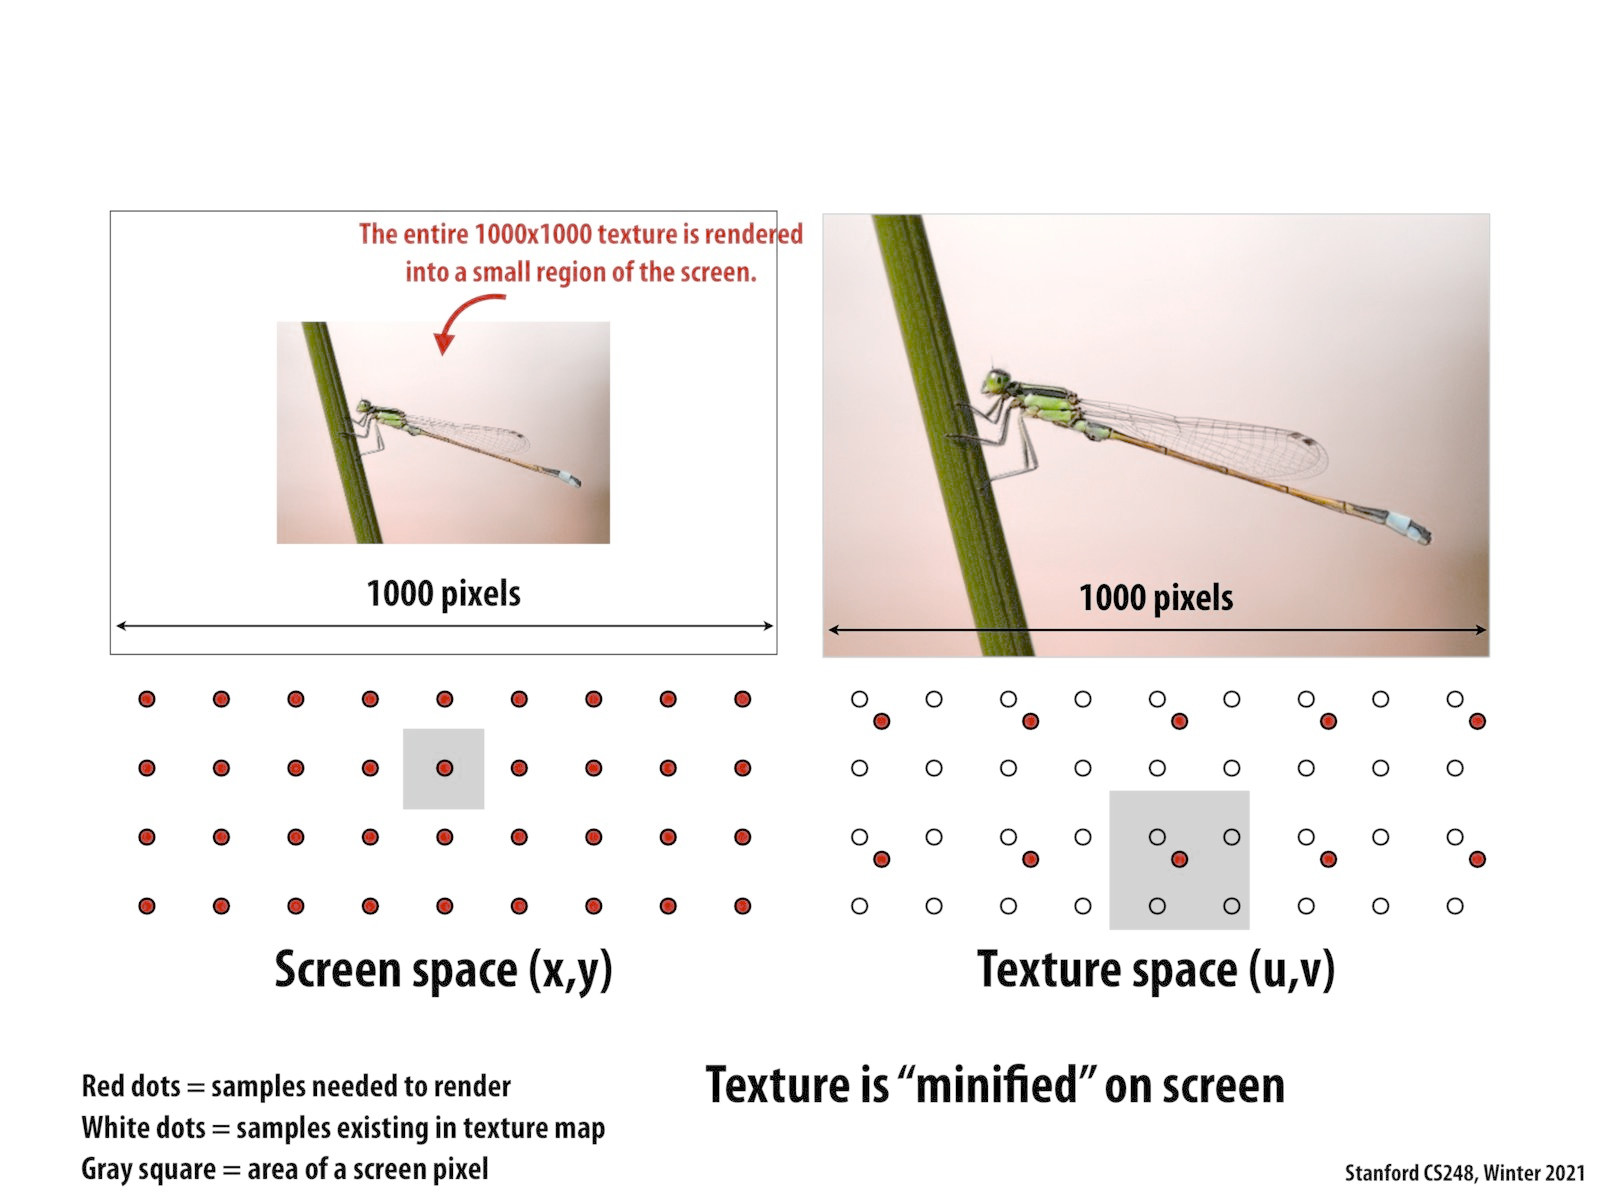
\includegraphics[width=10cm]{./slike/slide_051.jpg}
	\end{center}
\end{frame}

\begin{frame}{Teksture}
	\begin{center}
		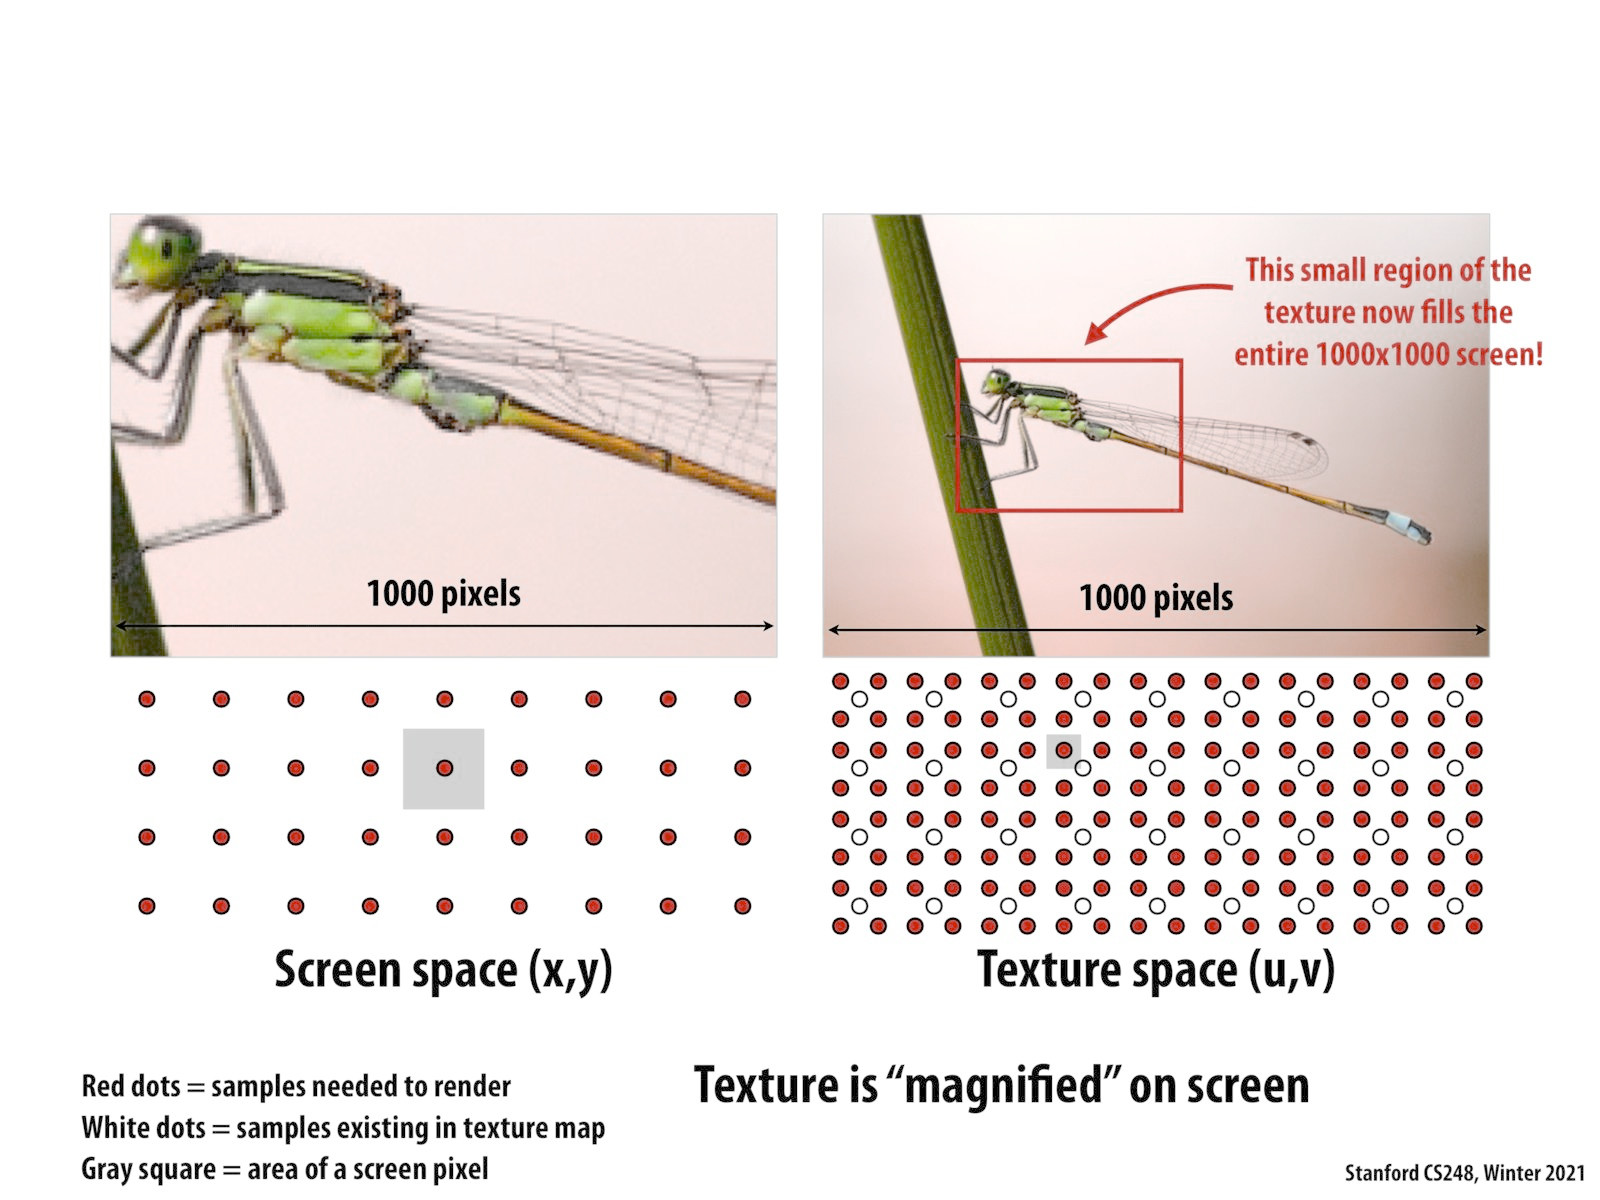
\includegraphics[width=10cm]{./slike/slide_052.jpg}
	\end{center}
\end{frame}

\begin{frame}{Teksture}
	\begin{center}
		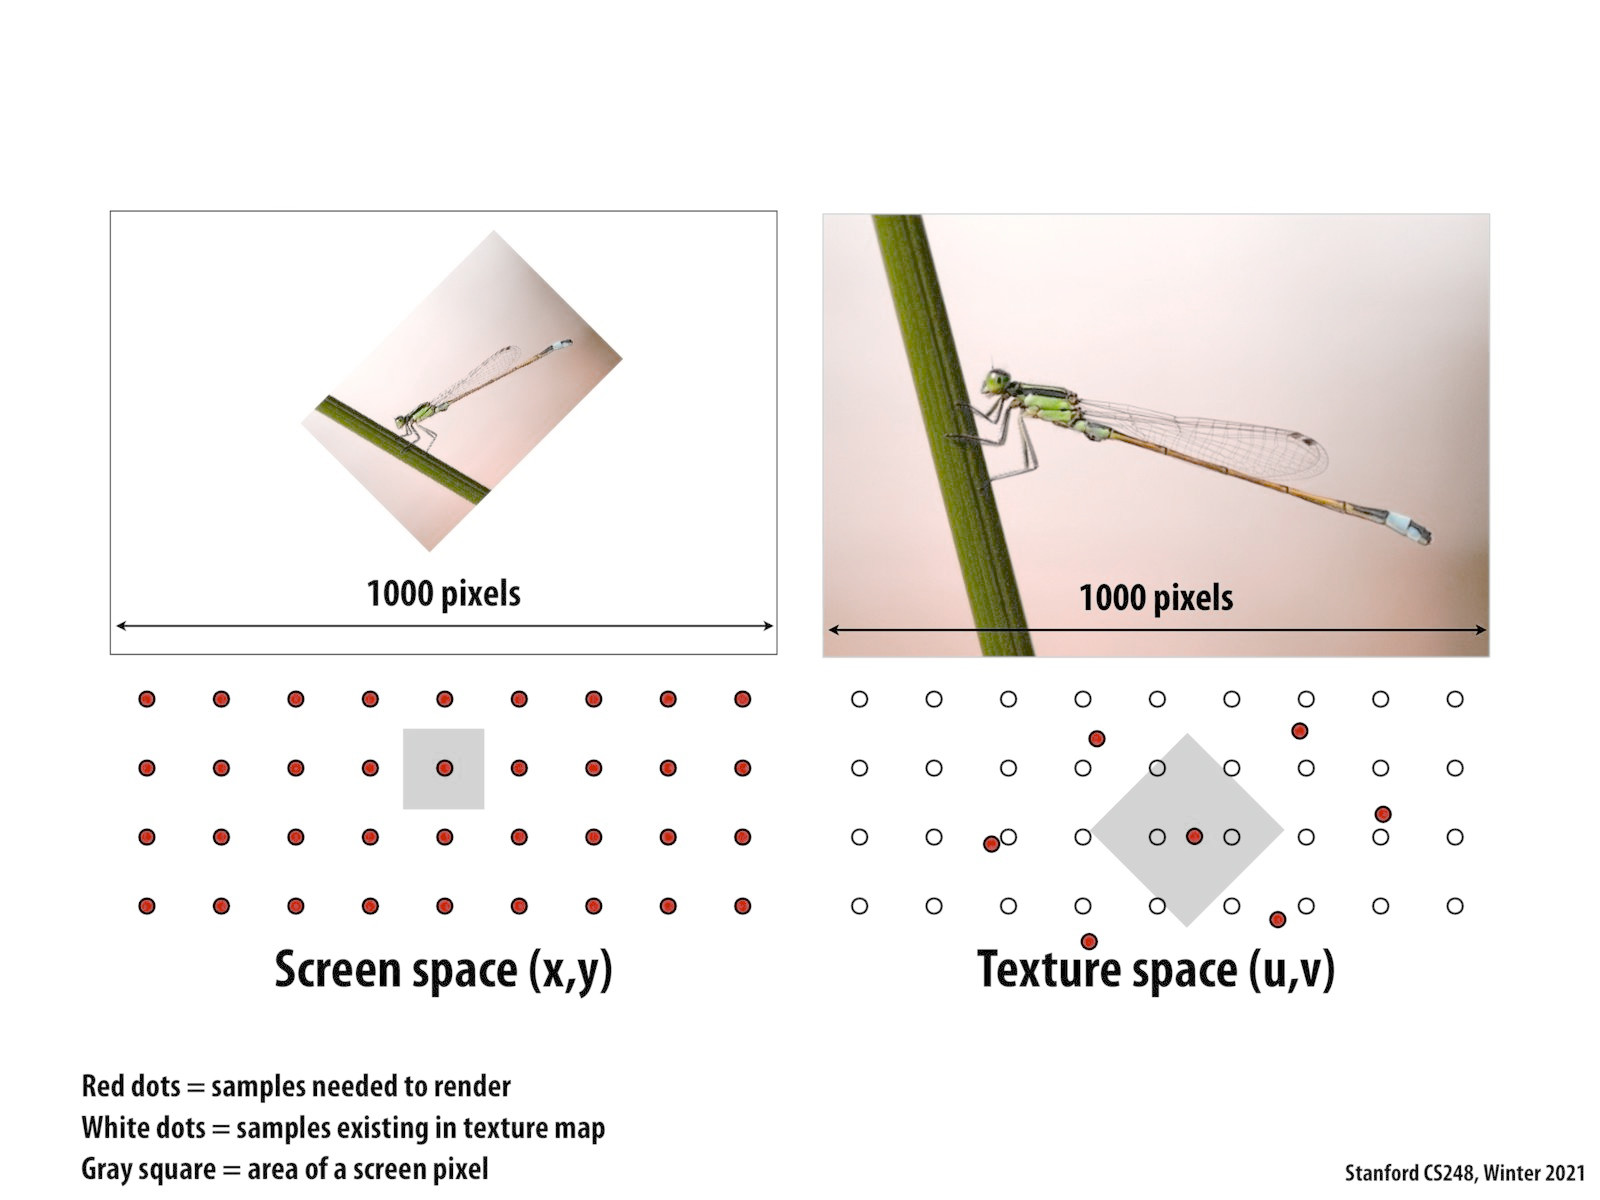
\includegraphics[width=10cm]{./slike/slide_053.jpg}
	\end{center}
\end{frame}

\begin{frame}{Teksture}
	\begin{center}
		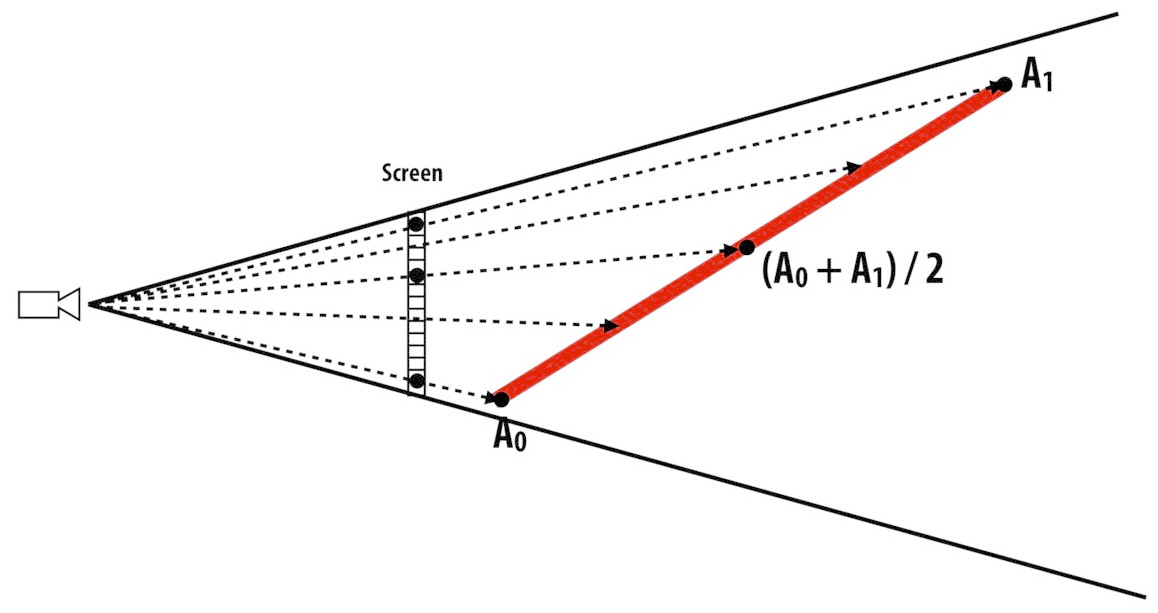
\includegraphics[width=5cm]{./slike/slide_030.jpg}
	\end{center}

	\begin{center}
		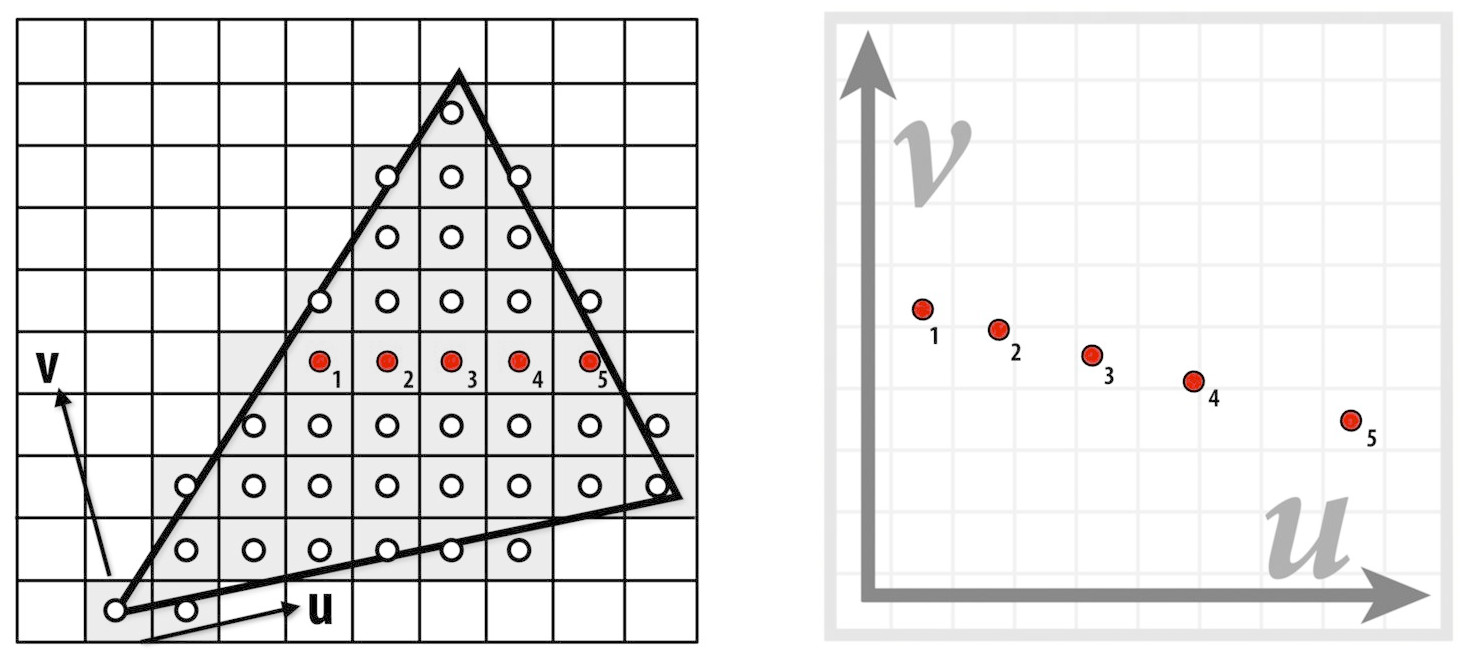
\includegraphics[width=6cm]{./slike/slide_054.jpg}
	\end{center}
\end{frame}

\begin{frame}{Teksture: magnification minification}
	\begin{itemize}
		\item Pri nekoj udaljenosti veličina piksela je jednaka texelu.
		\item Na manjoj udaljenosti texeli su veći od piksela te se moraju skalirati: \textit{magnification}
		\item Na većoj udaljenosti je texel manji od piksela, jedan piksel pokriva više texela, potrebno usrednjiti boju:
		\textit{minification}
	\end{itemize}
	\begin{center}
		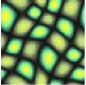
\includegraphics[width=1cm]{slike/teksture_mm_01.png} \hspace{0.5cm} 
		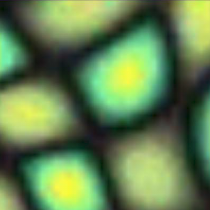
\includegraphics[width=3cm]{slike/teksture_mm_02.png} \hspace{0.5cm} 
		
\includegraphics[width=3cm]{slike/teksture_mm_03.png}
	\end{center}
\end{frame}
%
\begin{frame}{Kako odrediti boju piksela}
	\begin{itemize}
		\item Za zadane $(u,v)$ koordinate teksture, potrebno naći boju piksela u teksturi
	\end{itemize}
	\begin{center}
		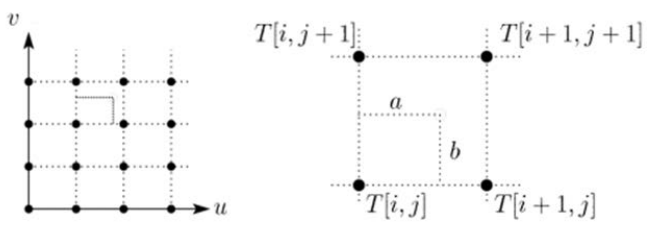
\includegraphics[width=8cm]{slike/pixel_rgb_color.png}
	\end{center}
	
\end{frame}
%\begin{frame}{Bilinearna interpolacija, opet}
%	\begin{center}
%		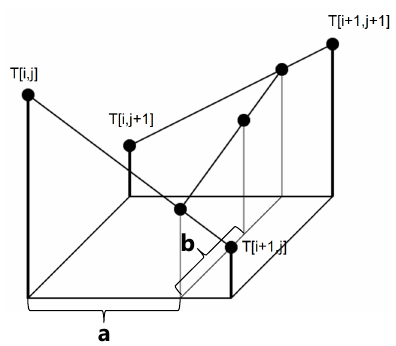
\includegraphics[width=6cm]{slike/bilinear_interpolation.png}
%	\end{center}
%\end{frame}
%
%\begin{frame}{Bilinearna interpolacija, opet}
%	\begin{center}
%		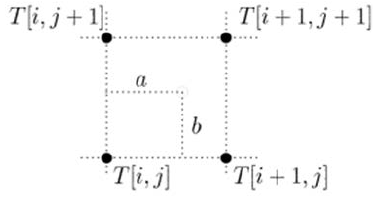
\includegraphics[width=6cm]{slike/bilinear_interpolation_close_up.png}
%	\end{center}
%	\begin{align*}
%	T(u, v) &= (1-a)(1-b)T[i, j] \\
%	&+ a(1-b)T[i+1, j] \\
%	&+ (1-a)bT[i, j+1] \\
%	&+ abT[i+1, j+1]
%	\end{align*}
%	\begin{itemize}
%		\item primjenjuje se za svaki R, G, B kanal s istim težinama
%	\end{itemize}
%\end{frame}
%
\begin{frame}{Učinak interpolacije}
	\begin{center}
		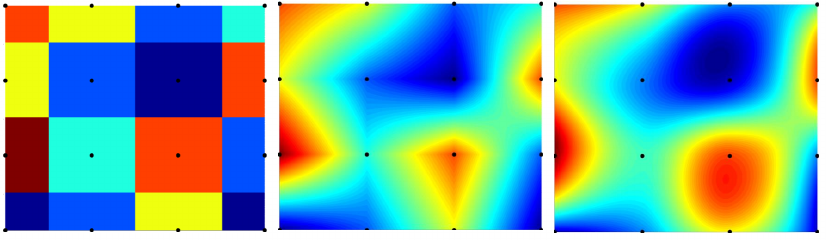
\includegraphics[width=10cm]{slike/teksture_magnification_01.png}
	\end{center}
\end{frame}
%
%
\begin{frame}{Alias učinak}
	
	\begin{center}
		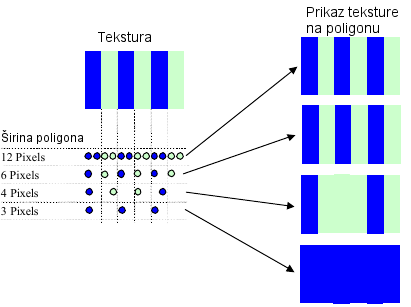
\includegraphics[width=7cm]{slike/04_alias_tekstura.png}
	\end{center}
\end{frame}
%
%\begin{frame}{Alias učinak contd.}
%	\begin{columns}[t]
%		\begin{column}{7cm}
%			\begin{block}{}
%				\begin{itemize}
%					\item Popunjavanjem poligona u ravnini se može \textit{promašiti} elemente strukture
%					\begin{itemize}
%						\item pre -fitriranje računa se prosječna vrijednost slikovnih elemenata strukture
%						\item povećano uzorkovanje (super sampling) po svakom slikovnom elementu u projekciji 
%						dohvaća 4 ili više elemenata strukture
%					\end{itemize}
%				\end{itemize}
%			\end{block}
%		\end{column}
%		\begin{column}{5cm}
%			\begin{center}
%				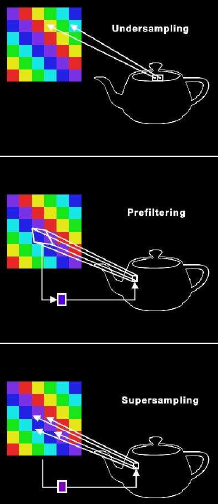
\includegraphics[width=2.8cm]{slike/05_sampling_tekstura.png}
%			\end{center}
%		\end{column}
%	\end{columns}
%\end{frame}
%
\begin{frame}{Mip mape}
	\begin{block}{}
		\begin{itemize}
			\item Originalna tekstura u visokoj rezoluciji se skalira i filtrira u više rezolucija unutar datoteke teksture. 
			\item MIP mape se mogu automatski generirati iz originalne teskture ili se mogu posebno izraditi.
			\item Obično svaki nivo je u pola manji od prethodnog, što garantira da kompletna tekstura nije veća 1.5 puta od originalne. Svaki sljedeći MIP nivo je obično duplo manji od prethodnog 
			\item Svaka skalirana tekstura predstavlja izgled teksture na određenoj udaljenosti od očišta. 
		\end{itemize}
	\end{block}
	\begin{center}
		\includegraphics[width=4.5cm]{slike/mipmap.png}
	\end{center}
\end{frame}
%
\begin{frame}{Mip mape contd.}
	\begin{block}{}
		\begin{itemize}
			\item Osnovna svrha jest očuvanje definicije teksture daleko od očišta i izbjegavanje moire-ovog efekta
			\item Kako se mip mape rade unaprijed, memorijski trošak je mali usporedi li se sa značajno unaprijeđenom kvalitetom 	
			slike
			\item MIP  - \textit{multum in parvo}, \small{mnoštvo u malom (prostoru)}.
		\end{itemize}
	\end{block}
	\begin{center}
		\includegraphics[width=3.5cm]{slike/06_mipmap_tekstura.png}
		\includegraphics[width=3.5cm]{slike/mip_mapa.png}
	\end{center}
\end{frame}


\begin{frame}{Tehnike uklanjanja neželjenih učinaka uzorkovanja}
	\begin{block}{}
		\begin{itemize}      
			\item Općenito tehnike uglađivanja stranica poligona
			\item Interpolacije - nearest neighbour, linearna, kubična, itd.
			\item Supersampling - tehnika prikupljanja točaka na većoj rezoluciji (obično 2x). Tada se napravi downsample, npr. prosječnom vrijednošću.
			\item Npr. Full scene anti alias sampling (FSAA) - svaka slika se renderira na 2x ili 4x rezoluciji i onda radi downsample na originalnu. 
			\item Multi sampling (MSAA) - optimirani supersampling, podržani u grafičkim karticama, malo slabija kvaliteta ali brže isrctavanje
		\end{itemize}
	\end{block}
\end{frame}
%
\begin{frame}{Preslikavanje okoliša - environment mapping}
	\begin{block}{}
		\begin{itemize}
			\item grafički protočni sustav ne dopušta zrcaljenje
			\item koriste se teksture i multipass algoritmi
			\item pretpostavlja se da je okoliš dovoljno daleko i da se objekt ne zrcali sam na sebe
		\end{itemize}
	\end{block}
	\begin{center}
		\includegraphics[width=5cm]{slike/terminator_2.png}
	\end{center}
\end{frame}

\section{Još primjena tekstura}
\begin{frame}{Posebne namjene}
	\begin{block}{Preslikavanje osvjetljenja}
		\begin{center}
			\includegraphics[width=6cm]{slike/teksture_light.png}
		\end{center}
		\begin{center}
			\includegraphics[width=6cm]{slike/teksture_light_02.png}
		\end{center}
	\end{block}
\end{frame}
%
\begin{frame}{Billboards}
	\begin{block}{Prozirne teksture}
		\begin{itemize}
			\item Preslikavanje teksture na poligon koji je uvijek okrenut prema promatraču (ili više
			statičnih poligona)
			\item Obično se koriste za prikaz drveća ($\alpha=0$ prozirno, $\alpha=1$ zeleno)
		\end{itemize}
	\end{block}
	\begin{center}
		\includegraphics[width=6cm]{slike/teksture_billboards_01.png}
	\end{center}
	\begin{center}
		\includegraphics[width=6cm]{slike/teksture_billboards_02.png}
	\end{center}
\end{frame}
%
\begin{frame}{Posebne namjene}
	
	\begin{block}{Stapanje tekstura uz zadane prozirnosti - $\alpha$ blending}
		\begin{itemize}
			\item Više slojeva koji imaju definiranu prozirnost
			\item Konveksna kombinacija boja - $C = c_{a}\alpha_{a}+ c_{b}\alpha_{b}(1-\alpha{a})$ 
			\item prozirnost - $\alpha = \alpha_{a}+ \alpha_{b}(1-\alpha{a})$ 
		\end{itemize}
	\end{block}
	\begin{center}
		\includegraphics[width=9cm]{slike/07_prozirnost.png}
	\end{center}
\end{frame}

\plain{Pitanja?}
\end{document}